%%% The main file. It contains definitions of basic parameters and includes all other parts.

% Meta-data of your thesis (please edit)
\input metadata.tex

% Generate metadata in XMP format for use by the pdfx package
\input xmp.tex

%% Settings for single-side (simplex) printing
% Margins: left 40mm, right 25mm, top and bottom 25mm
% (but beware, LaTeX adds 1in implicitly)
\documentclass[12pt,a4paper]{report}
\setlength\textwidth{145mm}
\setlength\textheight{247mm}
\setlength\oddsidemargin{15mm}
\setlength\evensidemargin{15mm}
\setlength\topmargin{0mm}
\setlength\headsep{0mm}
\setlength\headheight{0mm}
% \openright makes the following text appear on a right-hand page
\let\openright=\clearpage

%% Settings for two-sided (duplex) printing
% \documentclass[12pt,a4paper,twoside,openright]{report}
% \setlength\textwidth{145mm}
% \setlength\textheight{247mm}
% \setlength\oddsidemargin{14.2mm}
% \setlength\evensidemargin{0mm}
% \setlength\topmargin{0mm}
% \setlength\headsep{0mm}
% \setlength\headheight{0mm}
% \let\openright=\cleardoublepage

%% If the thesis has no printed version, symmetric margins look better
% \documentclass[12pt,a4paper]{report}
% \setlength\textwidth{145mm}
% \setlength\textheight{247mm}
% \setlength\oddsidemargin{10mm}
% \setlength\evensidemargin{10mm}
% \setlength\topmargin{0mm}
% \setlength\headsep{0mm}
% \setlength\headheight{0mm}
% \let\openright=\clearpage

%% Generate PDF/A-2u
\usepackage[a-2u]{pdfx}

%% Prefer Latin Modern fonts
\usepackage{lmodern}
% If we are not using LuaTeX, we need to set up character encoding:
\usepackage{iftex}
\ifpdftex
\usepackage[utf8]{inputenc}
\usepackage[T1]{fontenc}
\usepackage{textcomp}
\fi

%% Further useful packages (included in most LaTeX distributions)
\usepackage{amsmath}        % extensions for typesetting of math
\usepackage{amsfonts}       % math fonts
\usepackage{amsthm}         % theorems, definitions, etc.
\usepackage{bm}             % boldface symbols (\bm)
\usepackage{booktabs}       % improved horizontal lines in tables
\usepackage{caption}        % custom captions of floating objects
\usepackage{dcolumn}        % improved alignment of table columns
\usepackage{floatrow}       % custom float environments
\usepackage{graphicx}       % embedding of pictures
\usepackage{indentfirst}    % indent the first paragraph of a chapter
\usepackage[nopatch=item]{microtype}   % micro-typographic refinement
\usepackage{paralist}       % improved enumerate and itemize
\usepackage[nottoc]{tocbibind} % makes sure that bibliography and the lists
			    % of figures/tables are included in the table
			    % of contents
\usepackage{xcolor}         % typesetting in color

% The hyperref package for clickable links in PDF and also for storing
% metadata to PDF (including the table of contents).
% Most settings are pre-set by the pdfx package.
\hypersetup{unicode}
\hypersetup{breaklinks=true}

% Packages for computer science theses
\usepackage{algpseudocode}  % part of algorithmicx package
\usepackage{algorithm}
\usepackage{fancyvrb}       % improved verbatim environment
\usepackage{listings}       % pretty-printer of source code

% You might want to use cleveref for references
% \usepackage{cleveref}

% Set up formatting of bibliography (references to literature)
% Details can be adjusted in macros.tex.
%
% BEWARE: Different fields of research and different university departments
% have their own customs regarding bibliography. Consult the bibliography
% format with your supervisor.
%
% The basic format according to the ISO 690 standard with numbered references
\usepackage[natbib,style=iso-numeric,sorting=none]{biblatex}
% ISO 690 with alphanumeric references (abbreviations of authors' names)
%\usepackage[natbib,style=iso-alphabetic]{biblatex}
% ISO 690 with references Author (year)
%\usepackage[natbib,style=iso-authoryear]{biblatex}
%
% Some fields of research prefer a simple format with numbered references
% (sorting=none tells that bibliography should be listed in citation order)
%\usepackage[natbib,style=numeric,sorting=none]{biblatex}
% Numbered references, but [1,2,3,4,5] is compressed to [1-5]
%\usepackage[natbib,style=numeric-comp,sorting=none]{biblatex}
% A simple format with alphanumeric references:
%\usepackage[natbib,style=alphabetic]{biblatex}

% Load the file with bibliography entries
\addbibresource{bibliography.bib}

% Our definitions of macros (see description inside)
\input macros.tex

%%% Title page and various mandatory informational pages
\begin{document}
%%% Title page of the thesis and other mandatory pages

%%% Title page of the thesis

\pagestyle{empty}
\hypersetup{pageanchor=false}
\begin{center}

\centerline{\mbox{
\includegraphics[width=166mm]{../img/logo-en.pdf}}}

\vspace{-8mm}
\vfill

{\bf\Large BACHELOR THESIS}

\vfill

{\LARGE\ThesisAuthor}

\vspace{15mm}

{\LARGE\bfseries\ThesisTitle}

\vfill

\Department

\vfill

{
\centerline{\vbox{\halign{\hbox to 0.45\hsize{\hfil #}&\hskip 0.5em\parbox[t]{0.45\hsize}{\raggedright #}\cr
Supervisor of the bachelor thesis:&\Supervisor \cr
\noalign{\vspace{2mm}}
Study programme:&\StudyProgramme \cr
\noalign{\vspace{2mm}}
Study branch:&\StudyBranch \cr
}}}}

\vfill

% Zde doplňte rok
Prague \YearSubmitted

\end{center}

\newpage

%%% Here should be a bound sheet included -- a signed copy of the "bachelor
%%% thesis assignment". This assignment is NOT a part of the electronic
%%% version of the thesis. DO NOT SCAN.

%%% A page with a solemn declaration to the bachelor thesis

\openright
\hypersetup{pageanchor=true}
\pagestyle{plain}
\pagenumbering{roman}
\vglue 0pt plus 1fill

\noindent
I declare that I carried out this bachelor thesis independently, and only with the cited
sources, literature and other professional sources. It has not been used to obtain another
or the same degree.

\medskip\noindent
I understand that my work relates to the rights and obligations under the Act No.~121/2000 Sb.,
the Copyright Act, as amended, in particular the fact that the Charles
University has the right to conclude a license agreement on the use of this
work as a school work pursuant to Section 60 subsection 1 of the Copyright~Act.

\vspace{10mm}

\hbox{\hbox to 0.5\hsize{%
In \hbox to 6em{\dotfill} date \hbox to 6em{\dotfill}
\hss}\hbox to 0.5\hsize{\dotfill\quad}}
\smallskip
\hbox{\hbox to 0.5\hsize{}\hbox to 0.5\hsize{\hfil Author's signature\hfil}}

\vspace{20mm}
\newpage

%%% Dedication

\openright

\noindent
\Dedication

\newpage

%%% Mandatory information page of the thesis

\openright

\vbox to 0.5\vsize{
\setlength\parindent{0mm}
\setlength\parskip{5mm}

Title:
\ThesisTitle

Author:
\ThesisAuthor

\DeptType:
\Department

Supervisor:
\Supervisor, \SupervisorsDepartment

Abstract:
\Abstract

Keywords:
\Keywords

\vss}

\newpage

\openright
\pagestyle{plain}
\pagenumbering{arabic}
\setcounter{page}{1}


%%% A page with automatically generated table of contents of the thesis

\tableofcontents

%%% Each chapter is kept in a separate file
\chapter*{Introduction}
\addcontentsline{toc}{chapter}{Introduction}

\noindent
Anyone with internet access must have noticed the rapid development of artificial intelligence (AI). What used to be science fiction in the past (not that many years ago) is now becoming more and more relevant. Some people are fascinated and others are terrified by the capabilities of modern AI technologies, ranging from large language models (LLM) to generative video makers with precise details.

\medskip\noindent
We can have lengthy and deeply philosophical discussions on the definition and meaning of intelligence. Every living being has some kind of intelligence. Humans, animals, insects, and even trees have some level of intelligence and consciousness. We may not conclude on the final form of this definition, but surely we will all agree that a substantial part of intelligence is decision-making and planning. From the variety of all possible actions, we choose one that is the most suitable and optimal for the current situation. In situations where we want to attain a complex goal, we need to use our intelligence and create a plan, i.e., a sequence of valid actions that will change the current state of the world to the desired one.

\medskip\noindent
This thesis concerns the Hierarchical Task Network (HTN) which is the way most people think about problems and ways of solving them. Having some abstract and high-level tasks, we may decompose these tasks into subtasks that may be later again decomposed or executed right away. A high-level task is accomplished when all of its subtasks are accomplised. HTN can express different planning domains more compactly and intuitively than classical planning, which will be discussed in this thesis as well.

\section*{Motivation}

\noindent
The theory of classical and hierarchical planning is closely related to the theory of Automata~and~Grammars~\cite{complexity}~\cite{langclassification}~\cite{cmyk}. For this reason, we can utilize concepts, knowledge, and well-known structures from the theory of Automata~and~Grammars and apply them to the field of planning. Planning and especially hierarchical planning is widely used in AI and other similar fields of informatics.

\medskip\noindent
If we want to improve AI, then we need to improve planning, which is part of the concept of intelligence, as we discussed earlier. If we want to improve some theoretical knowledge, then we need to do theoretical research in that field. Hence, this bachelor's thesis was created, to at least somehow help the international community of researchers in this particular field. The impact will be most likely close to none, but it is important to remember the saying, "Rome was not built in a day".

\section*{Goal}

\noindent
\xxx{TODO}

\section*{Structure}

\noindent
In chapters one and two, we will describe and define classical planning and HTN planning, respectively. There are many different ways of representing both planning models, however, we will outline only the most known representations. In the third chapter, we will characterize various semantics of HTN planning. That is, what is the meaning of HTN models, and how we should think about them. Finally, the fourth chapter shows some transformations, that might help achieve prerequisites for particular HTN planners, for example, to compile away unsupported features.
\chapter{Classical {P}lanning}

\medskip\noindent
Before we dive into HTN planning, it's essential to understand its predecessor, which is classical planning or, as it is called in some literature, STRIPS planning~\cite{strips}. Classical planning is lightweight in the sense that it is easier to get into the theory of planning (independently on a representation of planning, which will be discussed in this chapter) and it is easier to describe domains of problems. The concept of classical planning is similar to the theory of Automata and Grammars (deterministic finite automaton (DFA), to be precise). There are different states of the world as well as actions that change one state to another. An action in classical planning can be viewed as a state transition function $\gamma: S \times A \rightarrow S$, where $S$ and $A$ denote the sets of all states and actions, respectively. If an action is applicable to a state then there will be a state transition, otherwise it will be undefined. The set of goal states, $S_g \subseteq S$, is analogous to a set of accepting states. The planning problem then can be reduced to a problem of searching paths in a directed graph.

\medskip\noindent
Although this approach of classical planning is simple and straightforward, it has one crucial flaw which makes it unusable in practice. Imagine a planning domain that describes a warehouse. If we have five locations, three piles of containers per location, three robots, and one hundred containers, then there are $10^{277}$ states~\cite{nau}, which is much more than the number of atoms in the observable universe. And that is just a simple small domain with a small amount of objects. For this purpose, we need to use better ways of representing classical planning, which will be called \emph{state-transition system}. We will briefly describe two possible representations: \emph{set-theoretic representation} and \emph{classical representation}.

\medskip\noindent
In both representations, the idea is to use more compact ways of defining a state of the world and actions that change the state. Instead of having a set of all states $S$, we will have a finite set of proposition symbols $P = \{p_1,\dots,p_n\}$ in \emph{set-theoretic representation} and a first-order language $\mathcal{L}$ in \emph{classical representation}. Both, $P$ and $\mathcal{L}$ describe properties and features of the world. Each state is then defined by a set of properties, which are true in that state and every other property is false. This feature is called closed world assumption. Both of these representations have the same expressive power~\cite{nau}. 

\medskip\noindent
All of the following definitions are correspondent and equivalent to the definitions in the book \emph{Automated Planning: theory and practice (Chapter 2)}~\cite{nau}.

\section{Set-Theoretic Representation}

\begin{defn}\label{def01:1}
  Let $P = \{p_1,\dots,p_n\}$ be a finite set of propositional symbols, which will model properties of a world. Then $\Sigma = (S, A, \gamma)$ is a \emph{planning domain} on $P$. $S$, $A$, and $\gamma$ denote the set of all states, set of all actions, and the \emph{state-transition function}, respectively, such that:

  \begin{itemize}
      \item $S \subseteq 2^{P}$, each state $s \in S$ holds in properties of the world, that are true. Other propositional symbols $p \in P$, $p \notin s$ do not hold in a state $s$.
      
      \item Each action $a \in A$ is defined as a triple of sets describing the preconditions and changes to a current state. Action $a \in A$ will be denoted as \mbox{$a=(pre(a), \text{eff}^{\,\,-}(a), \text{eff}^{\,\,+}(a)) \in  2^{P} \times 2^{P} \times 2^{P}$}, where $pre(a)$ stands for preconditions that must be true in a state to apply this action, meanwhile $\text{eff}^{\,\,-}(a)$ and $\text{eff}^{\,\,+}(a)$ describe changes to the state or, in other words, negative and positive effects\footnote{In some literature these sets are called: add list, delete list.}. We require $\text{eff}^{\,\,-}(a) \cap \text{eff}^{\,\,+}(a) = \emptyset$ for every $a \in A$, because otherwise it does not make any sense. Having a state $s \in S$, an action $a \in A$ is \emph{applicable} to state $s$, if and only if $pre(a) \subseteq s$ (it might be convenient to specify $pre^{-}(a)$ and $pre^{+}(a)$ to denote positive and negative preconditions).
      
      \item Having $s \in S$ and an action $a \in A$ that is \emph{applicable} to state $s$, \emph{state-transition} function $\gamma$ is defined as follows: $\gamma(s,a)=(s-\text{eff}^{\,\,-}(a)) \cup \text{eff}^{\,\,+}(a)$, otherwise it is undefined.
      \item $S$ must have a property that for every $s \in S$ and $a \in A$ that is \emph{applicable} to $s$, $\gamma(s,a) \in S$. This way we do not have to know all of the states in advance. All we need is a set of actions $A$ and some initial state $s_0 \in S$, then we can find all reachable states using Breadth-First Search (BFS), Depth-First Search (DFS), or some other searching algorithms.
  \end{itemize}
\end{defn}

\begin{defn}\label{def01:2}
  A \emph{planning problem} is a triple $\mathcal{P}=(\Sigma,s_o,g)$, such that:

  \begin{itemize}
    \item $\Sigma = (S, A, \gamma)$ is a \emph{planning domain} on $P$.
    
    \item $s_0 \in S$ is an \emph{initial state}.
    
    \item $g \subseteq P$ is a set of \emph{goal proposition symbol}, which must be true in the state after the final action of a plan. $S_g=\{s \in S | g \subseteq s\}$ is a set of goal states, i.e., states that satisfy the \emph{planning problem}~$\mathcal{P}.$
  \end{itemize}
\end{defn}

\noindent
Because the set of \emph{propositional symbol} $P$ is finite, sets of states, actions, and state-transition function are also finite.

\begin{defn}\label{def01:3}
  A \emph{plan} in a \emph{planning domain} $\Sigma$ is a finite sequence of actions $\pi=(a_1,\dots,a_k)$, where $k \geq 0$ and $(\forall a \in \pi) a \in A$. The \emph{plan} $\pi$ is \emph{applicable} to a state $s_0 \in S$, if and only if a sequence of states $(s_0,\dots,s_k)$ exist, such that: \mbox{$(1 \leq i \leq k)$} $s_{i-1} \subseteq pre(a_i)$ and $s_i = \gamma(s_{i-1},a_i) = ((s_{i-1}-\text{eff}^{\,\,-}(a_i)) \cup \text{eff}^{\,\,+}(a_i))$ is defined. Otherwise, the \emph{plan} $\pi$ is invalid. 

  \medskip\noindent
  In other words, a \emph{plan} $\pi=(a_1,\dots,a_k)$ is \emph{applicable} to a state $s_0$, if and only if a \emph{plan} $\pi'=(a_2,\dots,a_k)$ is \emph{applicable} to a state $s_1=\gamma(s_0,a_1) \in S$.

  \medskip\noindent
  Having a \emph{plan} $\pi=(a_1,\dots,a_k)$ and a state $s \in S$, we will abuse the notation to let $\gamma(s,\pi)$ denote a state $s_k \in S$, where we get after applying the sequence of actions of a plan, i.e.,
    \[
    \gamma(s,(a_1,\dots,a_k))=
    \begin{cases}
    s, & \text{if $k=0$ (there are no actions)},\\
    \gamma(\gamma(s,a_1),(a_2,\dots,a_k)), & \text{if k $>$ 0, $a_1$ is \emph{applicable} to $s$}, \\
    undefined, & \text{otherwise}.
    \end{cases}
    \]
\end{defn}



\begin{defn}\label{def01:4}
    A \emph{solution} to a \emph{planning problem} $\mathcal{P}=(\Sigma,s_o,g)$ is a plan $\pi=(a_1,\dots,a_k)$ that is \emph{applicable} to $s_0$, which changes the initial state $s_0$ to a state that satisfies \emph{goal propositional symbols}: $\gamma(s_0,\pi)$ is defined and $g \subseteq \gamma(s_0,\pi)$ (equivalent to $\gamma(s_0,\pi) \in S_g$).
\end{defn}

\noindent
For a \emph{planning problem} there might be many \emph{solutions}, moreover, there might be an infinite number of \emph{solutions} if there are states that can be visited repeatedly, (e.g. we might have two adjacent locations in a domain, that can be visited cyclically without any constraints).

\medbreak\noindent
It is easy to see that for each \emph{planning problem} $\mathcal{P}$ with nonempty set of \emph{solutions} (there exist a \emph{plan} $\pi$ such that $\pi$ is a solution to a $\mathcal{P}$) there exist at least one \emph{minimal solution} $\pi=(a_1,\dots,a_k)$, i.e., there is no \emph{solution} $\pi'=(a_1,\dots,a_j)$ such that $j < k$. There might be many different \emph{minimal solutions} but all of them share the same length.


\begin{example}\label{ex01:1}
    \begin{figure}
        \centering
        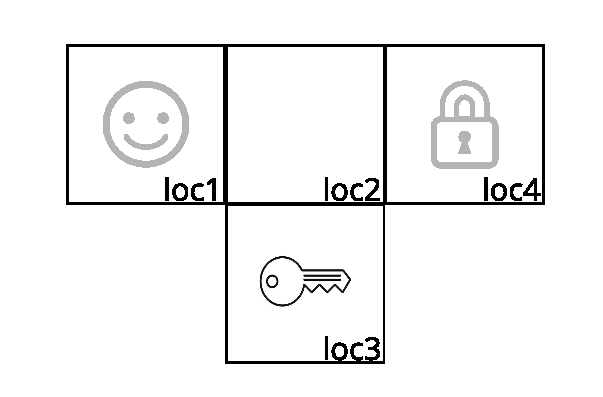
\includegraphics{img/output_mares_key1.pdf}
        \caption{Initial state of a simple planning domain}
        \label{fig01:1}
    \end{figure}
    
    Imagine a simple planning domain (Figure~\ref{fig01:1}) that can represent states in an uncomplicated maze-like game. We have four game locations, a player character, a key, and a locked door (illustrated by a \emph{loc4}). The character can move freely between locations but if he wants to enter \emph{loc4}, then he needs a key that can be picked at the \emph{loc3} (but cannot be discarded later on). Now we will define a planning problem $\mathcal{P}=(\Sigma,s_0,g)$ for this domain $\Sigma=(S,A,\gamma)$ more formally:
    
\end{example}

\begin{itemize}
    \item $P=\{${at-loc1,at-loc2,at-loc3,at-loc4,key-picked}$\}$,
    
    \item $S=\begin{aligned}[t]
    &\{\{ \mathrm{at\text{-}loc1}\}, \{ \mathrm{at\text{-}loc2}\}, \{ \mathrm{at\text{-}loc3}\}, \{ \mathrm{at\text{-}loc1,key\text{-}picked}\},\\
    & \{ \mathrm{at\text{-}loc2,key\text{-}picked}\},
    \{ \mathrm{at\text{-}loc3,key\text{-}picked}\}, \{ \mathrm{at\text{-}loc4,key\text{-}picked}\}\},
    \end{aligned}$

    \item $A=\begin{aligned}[t]
    &\mathrm{\{move12,move21,move23,move32,move24,move42,pick\}, where:} \\
    &\mathrm{move12 = (\{at\text{-}loc1\},\{at\text{-}loc1\},\{at\text{-}loc2\});} \\
    &\mathrm{move21 = (\{at\text{-}loc2\},\{at\text{-}loc2\},\{at\text{-}loc1\});} \\
    &\mathrm{move23 = (\{at\text{-}loc2\},\{at\text{-}loc2\},\{at\text{-}loc3\});} \\
    &\mathrm{move32 = (\{at\text{-}loc3\},\{at\text{-}loc3\},\{at\text{-}loc2\});} \\
    &\mathrm{move24 = (\{at\text{-}loc2,key\text{-}picked\},\{at\text{-}loc2\},\{at\text{-}loc4\});} \\
    &\mathrm{move42 = (\{at\text{-}loc4\},\{at\text{-}loc4\},\{at\text{-}loc2\});} \\
    &\mathrm{pick = (\{at\text{-}loc3\},\{\},\{key\text{-}picked\}),}
    \end{aligned}$ 

    \item $\gamma$ as defined in Definition~\ref{def01:1},

    \item $s_0 = \{ \mathrm{at\text{-}loc1}\}$ (Figure~\ref{fig01:1}),

    \item $g = \{ \mathrm{at\text{-}loc4, key\text{-}picked}\}$.
\end{itemize}

\noindent
Example~\ref{ex01:1} shows us a complete description of a \emph{planning domain} $\Sigma$ and a \emph{planning problem} $\mathcal{P}$. There is one and only \emph{minimal solution} which is $\pi=(\mathrm{move12,move23,pick,move32,move24})$. On the other hand, there is an infinite amount of \emph{solutions}. We might go to the loc3 and apply the action pick as many times as we desire, thus generating an infinite amount of \emph{solutions}.

\medskip\noindent
With knowledge of the particular domain, we can adjust the domain without losing any domain's specifics. For example, we might alter the set of the \emph{goal proposition symbols} $g$ to be $g=\mathrm{\{at\text{-}loc4\}}$ because we know that it is impossible to enter loc4 without having a key picked up at the loc3.

\medskip\noindent
The set of states $S$ contains all reachable states from the initial state $s_0$, other unreachable states might be added to the $S$ but they are not needed. For example, the state \{at-loc1,at-loc2\} is contradictory because we cannot be at two locations simultaneously. Likewise states \{\}, \{key-picked\}, \{at-loc4\} are also meaningless.

\medskip\noindent
The concept of the key in this domain is depicted as a \emph{propositional symbol} key-picked. This simplification does not take into account the location of a key because it is not needed in this domain. Once the key is picked, it will be implicitly located at the same location as the character. Hence, the action pick is \emph{applicable} more than once in a \emph{plan}.

\begin{figure}
    \centering
    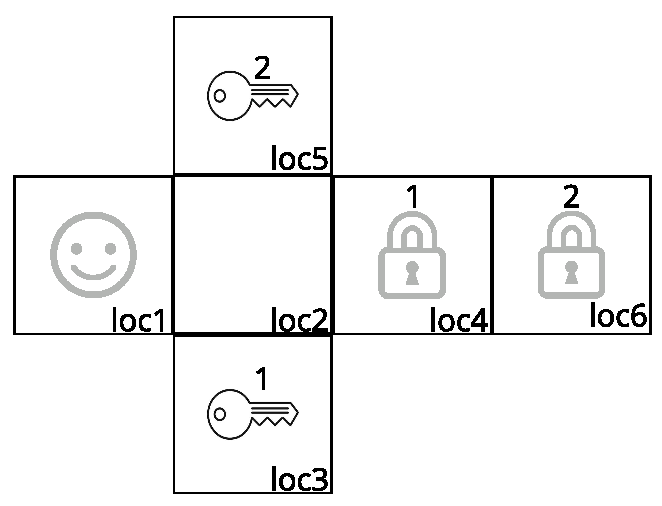
\includegraphics{img/output_mares_key2.pdf}
    \caption{Extended planning domain of a maze-like game}
    \label{fig01:2}
\end{figure}

\begin{example}\label{ex01:2}
    Let's consider an extension of this domain by adding two new locations, and another key (Figure~\ref{fig01:2}). Only this time we want to model a new constraint that allows at most one key to be held at a time. There are numerous ways of modeling this planning domain. For instance, we might introduce new \emph{propositional symbols}: \emph{key1-picked, key2-picked, door1-opened, door2-opened}. If we wanted to model the locations of keys, we would need to include many new \emph{propositional symbols} of the form \emph{key1-at-loc1, key1-at-loc2}, and so on. Also, we would need new \emph{actions} that would consider the locations of a key and the character. New actions may look like this: \emph{pick-key1-at1 = (\{at-loc1,key1-at-loc1\},\{key2-picked\},\{key1-picked\}), move12-with-key1 = (\{at-loc1,key1-at-loc1\},\{at-loc1,key1-at-loc1\},\{at-loc2,key1-at-loc2\})} and so on. This enumeration of possible substates might result in an enormous set of \emph{propositional symbols} and other related sets \emph{\cite{nau}~{(2.2.4 Properties of the Set-Theoretic Representation)}}. An elaborate solution that fixes this problem is discussed in the following chapter.
\end{example}

\section{Classical Representation}\label{class_repre}

\noindent
\emph{Classical representation} of planning improves \emph{set-theoretic representation} by introducing a first-order language $\mathcal{L}$ that consists of a finite number of constant symbols (similar to a set of \emph{propositional symbols} defined in Definition~\ref{def01:1}), predicate symbols, and other symbols for the representation of \emph{planning operators}. We do not allow any functional symbols in $\mathcal{L}$ because then we would have complications with modeling finite domains. A state in \emph{classical representation} is defined as a set of grounded logical atoms of $\mathcal{L}$.

\begin{example}\label{ex01:3}
    Before we start with definitions, we will look at Figure~\ref{fig01:1} from the perspective of \emph{classical planning}. We want to model the player, key, locations, and locked door. Thus, the set of constant symbols is \emph{\{player,loc1,loc2,loc3,loc4} \emph{,key1,nothing,door\}}. The constant symbol \emph{nothing} represents that the player's inventory is empty. With this knowledge, we can represent the initial state of Figure~\ref{fig01:1} to be $s_0=\{\mathrm{adjacent(loc1,loc2)},\mathrm{adjacent(loc2,loc1)},\mathrm{adjacent(loc2,loc3)}, \\ \mathrm{adjacent(loc3,loc2)}, \mathrm{adjacent(loc2,loc4)},\mathrm{adjacent(loc4,loc2)}, \mathrm{at(player,loc1)}, \\ \mathrm{holds(player,nothing)}, \mathrm{locked(door)}\}$. Some logical atoms will remain the same throughout all possible states, e.g. \emph{adjacent(loc1,loc2)}, meanwhile other atoms like \emph{at(player,loc1)} or \emph{holds(player,nothing)} will change after the application of proper actions.
\end{example}

\medskip\noindent
Now we will define \emph{planning operators} in \emph{classical planning}. \emph{Planning operators} do not contain any constant symbols, only variable symbols. A grounded instance of an operator is an action that can be part of a \emph{plan}.

\pagebreak

\begin{defn}\label{def01:5}
    A \emph{planning operator} is a triple $o = (name(o),precond(o), \\ \text{eff}(o))$, where:

        \begin{itemize}
            \item $name(o)$ is of a form $n(x_1,\dots,x_k)$, where $n$ is a \emph{operator symbol} and must be unique in $\mathcal{L}$ and $x_1,\dots,x_k$ represent variable symbols that appear in an operator,

            \item $precond(o)$ and $\text{eff}(o)$ generalize preconditions and effects of \emph{set-theoretic representation}. These sets contain positive and negative logical literals.
        \end{itemize}

    Let $O$ denote a set of all \emph{planning operators} as specified above.
\end{defn}

\medskip\noindent
In some literature, the usage of $name(o)$ is not specified, rather the multiset of grounded operators (actions) is assumed. The essence of $name(o)$ is in the planning phase. We might have multiple grounded instances of operators that might use the equivalent constant symbols. To help differentiate a \emph{planning operator} from an instance of a \emph{planning operator}, the $name(o)$ might come in handy. $name(o)$ refers unambiguously to one specific \emph{planning operator}. We will omit the usage $name(o)$ because the meaning will be obvious from the context.


\begin{example}\label{ex01:4}
    In this example, we will look at some possible \emph{planning operators} that might be used in Figure~\ref{fig01:2} (we will use new predicate symbols that were not specified yet):

    \begin{itemize}
        \item \emph{move(player,location1,location2)} \\
        precond: \emph{adjacent(location1,location2), at(player,location1), \neg locked(location2)} \\
        effects: \emph{\neg at(player,location1), at(player, location2)}

        \item \emph{pickup-key(player,key,location)} \\
        precond: \emph{at(player,location), at(key,location), holds(player,nothing)} \\
        effects: \emph{\neg holds(player,nothing), \neg at(key,location), holds(player,key)}

        \item \emph{drop-key(player,key,location)} \\
        precond: \emph{at(player,location), holds(player,key)} \\
        effects: \emph{\neg holds(player,key), at(key,location), holds(player,nothing)}

        \item \emph{open-door(player,location1,location2, key)} \\
        precond: \emph{adjacent(location1,location2), locked(location2), at(player,location1), key-opens-door(key,location2), holds(player,key)} \\
        effects: \emph{\neg locked(location2)}
    \end{itemize}
\end{example}

\medskip\noindent
In the Example~\ref{ex01:4} predicate symbols adjacent(l1,l2) and key-opens-door(key,location) are describing static properties of a domain that will never change and thus, will never appear in effects of \emph{planning operators}. On the other hand, predicate symbols like at(player/key,location), locked(location), or holds(player, key) will change and therefore will occur in effects of \emph{planning operators}.

\begin{defn}\label{def01:6}
Let us be given a state $s \in S$ and an action (ground instance of a \emph{planning operator}) $a$. If $precond^{+}(a) \subseteq s$ and $precond^{-}(a) \cap s = \emptyset$, where $precond^{+}(a)$ denotes a set of all positive atoms in $precond(a)$ and $precond^{-}(a)$ denotes a set of all atoms whose negation is in $precond(a)$, then $a$ is \emph{applicable} to $s$ and $\gamma(s,a)=(s-\text{eff}^{\,\,-}(a)) \cup \text{eff}^{\,\,+}(a)$. $\text{eff}^{\,\,-}(a)$ and $\text{eff}^{\,\,+}(a)$ are analogous to $precond^{-}(a)$ and $precond^{+}(a)$, respectively.
\end{defn}

\begin{defn}\label{def01:7}
Having a first-order language $\mathcal{L}$ with a finite amount of constant and predicate symbols and no functional symbols, the \emph{classical planning domain} in $\mathcal{L}$ is a state-transition system $\Sigma = (S,A,\gamma)$ such that:

    \begin{itemize}
        \item $S \subseteq 2^{\displaystyle \{all~ground~atoms~of~\mathcal{L}\}}$,
        
        \item $A =~$\{all ground instances of operators in $O$\},
        
        \item $\gamma$ is analogous Definition~\ref{def01:1},
        
        \item $S$ is closed under $\gamma$ in the same manner as in Definition~\ref{def01:1}.
    \end{itemize}
\end{defn}

\begin{defn}\label{def01:8}
A \emph{classical planning problem} is corresponding to \emph{set-theoretic planning problem}, it is defined as $\mathcal{P} = (\Sigma,s_0,g)$, where:

    \begin{itemize}
        \item $\Sigma = (S,A,\gamma)$ is a \emph{classical planning domain},
        
        \item $s_0 \in S$ is an initial state
        
        \item $g$ is a set of literals.
    \end{itemize}
\end{defn}

\chapter{Hierarchical {P}lanning}

\medskip\noindent
Now that we have understood classical planning, we can move on to hierarchical planning or Hierarchical Task Network (HTN), to be precise. In HTN the goal alone is not to find an \emph{applicable plan} that will meet all of the criteria of the \emph{planning problem}. HTN focuses on accomplishing some set of tasks by decomposing them into sub-tasks with constraints like ordering and state conditions. A task is accomplished immediately upon all of his sub-tasks are accomplished. HTN is an extension of classical planning which gives us clues on how to find the proper \emph{plan}.

\medskip\noindent
As in classical planning, there are states of the world represented by the set of \emph{proposition symbols} or \emph{logical atoms} that are true in a state. We can \emph{apply actions} to states if the preconditions of \emph{actions} are satisfied (held in a state). These \emph{actions} will be called \emph{primitive tasks} in HTN. These tasks are executable right away and they change the current state to another one by applying negative and positive effects. In addition to \emph{primitive tasks} there are \emph{non-primitive tasks}. We will call them \emph{compound tasks}. These tasks cannot be executed and \emph{applied to a state}, rather they have to be decomposed into a set of sub-tasks using decomposition \emph{methods}, both \emph{primitive} and \emph{compound}. Having an \emph{initial task network}, that is a set of tasks and a set of constraints, the goal is to decompose all tasks into \emph{primitive tasks} and find an ordering of these tasks so that the constraints are not violated. After doing so, it is important to check that the resulting \emph{plan} (a sequence of \emph{primitive tasks}) is a valid \emph{plan} and can be \emph{applied} to an \emph{initial state}.

\medskip\noindent
All of the following definitions are correspondent and equivalent to the definitions in the book \emph{Automated Planning: theory and practice (Chapter 11)}~\cite{nau} and other publications~\cite{langclassification}~\cite{cmyk}~\cite{ondrckova2023semantics}~\cite{ondrckova2024empty}.

\section{HTN Planning}

\begin{defn}\label{def02:9}
    A \emph{task network} is a pair $\omega = (U,C)$, where $U$ is a set of \emph{tasks} (primitive and compound) and $C$ is a set of constraints.
    
    For a \emph{solution} (\emph{plan}) to be valid we need to satisfy all of the constraints listed in $C$. We identify four types of constraints:

    \begin{itemize}
        \item $t_i \prec t_j$ where $t_i,t_j \in U$: an \emph{ordering-constraint} meaning that in every valid \emph{solution} the last \emph{primitive task} (\emph{action}) in the \emph{solution} to which $t_i$ decomposes must precede the first \emph{primitive task} (\emph{action}) in the \emph{solution} to which $t_j$ decomposes,
        
        \item $before(l,U')$: \emph{before-constraint} symbolizing that in every valid \emph{solution} the literal $l$ must hold in a state right before the \emph{application} of a first \emph{action} to which $U' \subseteq U$ decomposes,
    
        \item $after(U',l)$: \emph{after-constraint} is similar to \emph{before-constraint} with the difference that the literal $l$ must hold in a state right after the last \emph{action} to which set $U'$ decomposes,
    
        \item $between(U',l,U'')$: \emph{between-constraint} is saying that the literal $l$ must hold in all states starting after the last \emph{action} of $U'$ and lasting until the state right before the \emph{application} of a first \emph{action} of $U''$.
    \end{itemize}

    We will say that the \emph{task network} is \emph{primitive} if and only if, all of the tasks are \emph{primitive}. A \emph{task network} having at least one \emph{compound task} will be called \emph{non-primitive}.
\end{defn}

\medskip\noindent
The most used \emph{state-constraint} is \emph{a before-constraint} which can be modeled in various HTN planners. The usage and application of this constraint is obvious. Before the beginning of a task, we want to hold some preconditions that are significant for that particular task. For example, a user needs to input all of the information before he can continue with the paying; a player needs to complete all of the quests before he can move on to the next stage, or a warehouse robot needs to have permission set before he can execute some real-life tasks. Analogous \emph{after-constraint} has different use cases. We might use this constraint on the last task in \emph{the task network} to signalize our intentions which are not modeled with the tasks themselves. For example, we want to deallocate resources of the process after the completion, or we want to give a player new abilities after the completion of many tasks that might interleave. This constraint can be used as a shortcut in difficult models where the person responsible for the modeling cannot enumerate and decide the ordering of tasks perfectly. \emph{The between-constraint} represents an interval of states which hold some property. For example, we want a player to have a specific item in his inventory after the completion of one task and lasting until the other tasks, or an autonomous robot must hold a crate in all states meanwhile he moves from one location to another (possibly doing other unrelated things).

\medskip\noindent
In accordance with the Definition~\ref{def01:5}, the more formal definition~\cite{complexity}~\cite{langclassification}~\cite{nau} of the \emph{task network} would contain some function $\alpha: U \rightarrow N$, which would map instances of \emph{primitive} and \emph{compound tasks} to the set of names of all \emph{tasks}. This function would allow us to have multiple instances of the same \emph{task} in the set of tasks $U$, each with a unique identifier. We will omit a function $\alpha$ because its context will always be clear.

\begin{defn}\label{def02:10}
    A \emph{method} is a triple $m = (compound(m),subtasks(m), \\ constraints(m))$, where $compound(m)$ is a \emph{compound  task} and $(subtasks(m), \\ constraints(m))$ is a \emph{task network}. $constraints(m)$ operate only with the tasks in $subtasks(m)$. Having a \emph{task network} $\omega=(U,C)$, \emph{compound task} $c \in U$, and an instance of \emph{method} $m$ from $M$. Then $m$ decomposes $c$ into $subtasks(m)$, creating a new \emph{task network} $\omega'=(U',C')$ of a form:

    \[
    \delta(\omega,c,m) = ((U-\{c\}) \cup subtasks(m), C' \cup constraints(m)),
    \]

    \noindent
    where $C'$ is a modification of $C$:

    \begin{itemize}
        \item replace each \emph{ordering-constraint} containing $c$ with new ones containing $subtasks(m)$, i.e., $\forall c' \in subtasks(m): c \prec x$ is replaced with $c' \prec x$ and $x \prec c$ is replaced with $x \prec c'$,
        
        \item replace each \emph{before-, after-, between-constraint} containing $c$ with new ones containing $subtasks(m)$. For example, we would replace \emph{before-constraint} $before(l,V)$ with $before(l,(V - \{c\}) \cup subtasks(m))$.
    \end{itemize}
\end{defn}

\medbreak\noindent
It is highly convenient to write planning \emph{methods} as rewriting rules~\cite{ondrckova2023semantics}:

\[
T \rightarrow T_1,\dots,T_k \quad [C].
\]

\noindent
This rewriting rule symbolizing a \emph{method} is saying as follows: A \emph{method} which decomposes the \emph{compound task} $T$ into sub-tasks $T_1,\dots,T_k$ under the constraints $C$.

\medbreak\noindent
Definition~\ref{def02:10} works well for \emph{planning domains} without \emph{empty methods} (a \emph{method} that decomposes compound task into the empty set of subtasks). Using \emph{an empty method} creates undefined behavior because the decomposed compound task is removed from all constraints and thus it is unclear where the specified constraint should be checked. For this reason, we will later redefine \emph{method} decomposition. 

\begin{defn}\label{def02:11}
    A \emph{(HTN) planning domain} is a quadruple $\mathcal{D} = (\mathcal{L} \ / \ P, O, C, M$), where $\mathcal{L} \ / \ P$ and $O$ are first-order language (\emph{set of propositional symbols}) and a set of \emph{operators}, respectively, as described in the section \nameref{class_repre}, $C$ is a set of \emph{compound tasks} and $M$ represents a set of all \emph{methods}.

    \noindent
    \emph{Planning domain} will be referred to as \emph{totally-ordered} if all of the \emph{methods} in $M$ and the \emph{initial task network} are \emph{totally-ordered} (there is a total strict ordering of sub-tasks). \emph{Planning domains} that are not \emph{totally-ordered} will be referred to as \emph{partially-ordered}.
\end{defn}

\medskip\noindent
A first-order language $\mathcal{L}$ can be easily interchanged for a set of \emph{propositional symbols} $P$ due to the equivalent expressive power of \emph{set-theoretic representation} and \emph{classical representation}~\cite{nau}.

\begin{defn}\label{def02:12}
    A \emph{(hierarchical) planning problem} is a triple $\mathcal{P} = (s_0,\omega,\mathcal{D})$ that consists of \emph{initial state} of the world $s_0$, \emph{initial task network} $\omega$ and a \emph{planning domain} $\mathcal{D}$.
\end{defn}

\begin{defn}\label{def02:13}
    A \emph{solution} to the \emph{planning problem} $\mathcal{P}$ is a \emph{plan} $\pi=(a_1,\dots,a_k)$. This sequence of \emph{actions} is assembled from a \emph{primitive task network} $\omega'=(U', C'), \; U' = 
 \{a_i \; | \; 1 \leq i \leq k\}$, after the application of a sequence of \emph{methods} from $M$ to the \emph{initial task network} $\omega$. A \emph{solution} $\pi$ needs to be valid, i.e., $\gamma(s_0,\pi)$ is not undefined and also needs to satisfy all of the constraints in $C'$. That is:
    
    \begin{itemize}
        \item $a_i \prec a_j \implies i < j$,
        
        \item $before(l, V) \implies l \in s_{min\{i \; | \; a_i \; \in \; V\} \; - \; 1}$ (if the literal $l$ is negative then it must not be in a state, same applies for other constraints),
        
        \item $after(V,l) \implies l \in s_{max\{i \; | \; a_i \; \in \; V\}}$,
        
        \item $between(V',l,V'') \implies (\forall j, \; max\{i \; | \; a_i \; \in \; V'\} \; \leq \; j \; < \; min\{i \; | \; a_i \; \in \; V''\}: l \; \in \; s_j)$.
    \end{itemize}
    
    By $l$ we mean a ground instance of a literal $l$ (in the case of \emph{set-theoretic} representation it would be $p \in P$).
\end{defn}

\section{HTN and Context-free Grammars}

\medskip\noindent
With the knowledge acquired in the previous sections, we can try to map planning definitions and structures to the definitions and structures of the theory of Automata and Grammars. By doing so, we would be able to utilize already discovered knowledge and algorithms. Furthermore, it will allow us to prove different language classifications~\cite{langclassification}.

\medskip\noindent
The simplest example is to map \emph{classical planning problem} to the equivalent DFA, and vice versa. The mapped DFA generates all of the \emph{solutions}, i.e., \emph{plans} that are valid, \emph{applicable} to the \emph{initial state} $s_0$ and satisfy the goal $g$.

\begin{thm}\label{thm02:1}
    For every \emph{classical planning problem $\mathcal{P} = (S, A, \gamma, s_0, g)$}, where $(S, A, \gamma)$ is a \emph{planning domain}, there exists a DFA~\cite{chytil} $D = (Q, \Sigma, \delta, q_0, F)$ such that $D$ generates all the \emph{solutions} for $\mathcal{P}$.
\end{thm}
\begin{proof}
    The proof is straightforward. Having $\mathcal{P} = (S, A, \gamma, s_0, g)$, we can construct DFA $D = (S,A,\delta,s_0,S_g)$ where $S_g=\{s \in S | g \subseteq s\}$ and $\delta(s,a) = \gamma(s, a) = (s-\text{eff}^{\,\,-}(a)) \cup \text{eff}^{\,\,+}(a)$. We can easily see that every generated word (\emph{plan}) $\pi \in L(A)$ is also a valid \emph{solution} to the \emph{planning problem}. Every \emph{solution} is \emph{applicable} to the $q_0 = s_0$ because \emph{transition function} of $D$ imitates \emph{planning state-transition function} of $\mathcal{P}$. Every $\pi \in L(A)$ is a \emph{solution} because the set of accept states is $S_g$.
\end{proof}

\begin{thm}\label{thm02:2}
    For every DFA $D = (Q, \Sigma, \delta, q_0, F)$ there exists a correspondent \emph{classical planning problem $\mathcal{P} = (S, A, \gamma, s_0, g)$} where the set of \emph{solutions} of $\mathcal{P}$ is equal to $L(D)$.
\end{thm}
\begin{proof}
    Having DFA $D = (Q, \Sigma, \delta, q_0, F)$, we will construct \emph{planning problem} $\mathcal{P}$ with individual components defined as follows. Without loss of generality, we will rename states of $Q$. Each state $q \in Q$ will have a unique index $i$: $0 \leq i < |Q|$. $q_0$ is the \emph{initial state} of $D$. Now we define $\mathcal{P} = (S, A, \gamma, s_0, g)$ with:

    \begin{gather*}
        S = \{{\{i\} | q_i \in Q - F}\} \cup \{{\{i, goal\} | q_i \in F}\}, \\
        A = \{ \sigma = ( \{i\}, \{i, goal\}, \{j\} ) | \delta(q_i,\sigma) = q_j \; and \; q_j \notin F\} \cup \\ \{ \sigma = ( \{i\}, \{i\}, \{j, goal\} ) | \delta(q_i,\sigma) = q_j \; and \; q_j \in F\}, \\
        \gamma(s,a)=(s-\text{eff}^{\,\,-}(a)) \cup \text{eff}^{\,\,+}(a), \\
        s_0 = 
            \begin{cases}
                $\{0\}$, & \text{if $q_0 \notin F$},\\
                $\{0, goal\}$, & \text{if $q_0 \in F$},
            \end{cases} \\
        g = \{ goal \}.
    \end{gather*}

    Every generated word $\sigma_1\dots\sigma_n \in L(D)$ corresponds to a single \emph{solution} $\pi = (a_1, \dots, a_n)$. Each state of $\mathcal{P}$ is represented by an index (\emph{propositional symbol}) $i$ which specifies the state $q_i \in Q$. If a state is an accepting state, then the planning state $s$ has \emph{propositional symbol} $goal$. This is forced by the positive and negative effects of \emph{actions}.
\end{proof}

\begin{cor}\label{cor2:1}
    Classical planning is classified into the class of regular languages.
\end{cor}

\medskip\noindent
Now we will prove that \emph{totally-ordered} HTN planning can be represented as a context-free (CF) grammar and vice versa. These claims are extremely useful and will be used in the following parts of this thesis. Similar proofs are presented in~\cite{langclassification}.

\begin{thm}\label{thm02:3}
    For every CF grammar $G = (V_G, T_G, P_G, S_G)$~\cite{chytil} there exists a correspondent \emph{totally ordered planning problem} $\mathcal{P} = (s_0,\omega,\mathcal{D})$ with $\mathcal{D}=(P, O, C, M)$ such that the set of \emph{solutions} of $\mathcal{P}$ is equal to $L(G)$.
\end{thm}
\begin{proof}
    Constructing \emph{planning problem $\mathcal{P}$} is uncomplicated and intuitive because the structures are similar. All we need is to handle \emph{operators $o \in O$} so that the generated \emph{plans} are \emph{applicable} to the \emph{initial state} $s_0$. Having $G = (V_G,T_G,P_G,S_G)$ we construct $\mathcal{P} = (\{\}, (\{S_G\}, \{\}), \mathcal{D})$ with $\mathcal{D} = (\{\},T_G,V_G,M)$. \emph{Methods} are defined as follows:
    
    \[
    M = \{T \rightarrow T_1,\dots,T_k \; [ \; \{T_i \prec T_j \; | \; 1 \leq i < j \leq k\} \; ] \; | \; (T,T_1 \dots T_k) \in P_G\}.
    \]
    
    Using this construction, the \emph{planning problem $\mathcal{P}$} can now generate the set of \emph{plans} that equals $L(G)$. One problem is that the generated \emph{plans} might not be valid \emph{solutions}. This can be handled conveniently if we use empty sets for the preconditions of all \emph{operators}. Each $o \in O$ will be defined as $o = (\{\}, \{\}, \{\})$. The result of this modification is that every possible \emph{plan} is now a valid \emph{solution} if it can be decomposed from the \emph{initial task network}.
\end{proof}

\begin{thm}\label{thm02:4}
    For every \emph{totally ordered planning problem} $\mathcal{P} = (s_0,\omega,\mathcal{D})$ with $\mathcal{D}=(P, O, C, M)$ without \emph{before-, after-, between-constraints} there exists a CF language $L$ that is equal to the set of \emph{solutions} of $\mathcal{P}$.
\end{thm}
\begin{proof}
    Let $\mathcal{P} = (s_0,\omega = (U, C), \mathcal{D} = (P, O, C, M))$ be a \emph{totally ordered planning problem} in which constraints of each \emph{method} consist only of \emph{ordering-constraints}. We will construct CF grammar $G = (V_G, T_G, P_G, S_G)$ where $V_G = C, T_G = O$ and $S_G \in U$. We assume that the \emph{initial task network} $\omega$ consists of one task, $|U| = 1$. If there are more tasks (that are totally ordered by constraints $C$), we will add one extra production rule to the $P_G$ that rewrites the new starting symbol $S'_G$ to the given state of $\omega = (U, C)$. The set of production rules is defined as follows:
    
    \[
    P_G = \{(T, T_1\dots T_k) \; | \; (T, \{T_1, \dots, T_k\}, \{T_i \prec T_j \; | \; 1 \leq i < j \leq k\}) \in M\}.
    \]

    Grammar $G$ generates all \emph{plans} that can be generated with $\mathcal{P}$. Some of these \emph{plans} might be valid \emph{solutions} and some of them might not be \emph{applicable} to the \emph{initial state} $s_0$. In other words, $L(G)$ is a superset of all possible \emph{solutions} of $\mathcal{P}$. To solve this issue it is sufficient to use the fact that the intersection of a context-free language and a regular language is resulting into context-free language~\cite{chytil}. We can use Theorem~\ref{thm02:1} to build a DFA $D$ that will generate all \emph{plans} that are \emph{applicable} to $s_0$. The empty set of goal symbols $g = \emptyset$ will ensure that the language of $D$ equals to all possible \emph{plans} that are allowed by the planning \emph{operators} $O$. Having everything prepared, we can construct a CF language $L = L(G) \cap L(D)$ which is equal to the set of \emph{solutions} of $\mathcal{P}$.
\end{proof}

\begin{cor}\label{cor2:2}
Totally-ordered HTN planning without state-constraints is classified into the class of context-free languages.
\end{cor}

\section{HTN Plan Verification}

\medskip\noindent
Hierarchical plan verification can be seen as a reversal process to the decomposition of a \emph{initial task network} into a \emph{plan} that is \emph{applicable} to the \emph{initial state} $s_0$ and satisfies all constraints. Given a \emph{hierarchical planning domain} $\mathcal{D} = (P, O, C, M)$, \emph{initial task network} $\omega$, an \emph{initial state} $s_0$, and a \emph{plan} $\pi$, we ask if it is possible to decompose the $\omega$ into $\pi$ using $\mathcal{D}$. Depending on a hierarchical model or semantics specification, there might be some additional information and structures to the input of a plan verification problem. An approach for totally-ordered plan verification with \emph{method} preconditions is discussed here~\cite{cmyk}.       
\chapter{{HTN} Semantics}

\medskip\noindent
So far we have only discussed the definitions of classical and hierarchical planning. In this chapter, we will consider various semantics for hierarchical planning. A large part of this chapter will compare and describe semantics concerning \emph{empty methods} which are not defined properly within Definition~\ref{def02:10}. The main issue regarding \emph{empty methods} is caused by the unclear and ambiguous modification of \emph{task network's} constraints. It is uncertain how and when the modified constraints need to be checked. In the first part of this chapter, we will analyze existing approaches and propose new ways of handling \emph{empty methods} concerning the HTN plan verification process. In the second part, we will introduce a new idea for modeling hierarchical planning problems without the negative effects of \emph{primitive tasks}.

\section{Empty Methods}

\medskip\noindent
The following section will describe different solutions of how to handle \emph{empty methods}.

\begin{example}\label{ex03:5}
    \xxx{motivate pro pouziti prazdnych method v praxi}
\end{example}

\begin{example}\label{ex03:6}
    Suppose we have a simple \emph{task network} $\omega = (\{t1, t2\}, \{t1 \prec t2, \\ before(p, t2)\})$. In natural language, we would say that task (\emph{primitive} or \emph{compound}) $t1$ must precede task $t2$, and at the same time, before executing the first \emph{primitive task} to which task $t2$ decomposes (in case of a \emph{primitive task}, we mean the state before the \emph{application} of the task $t2$) the \emph{propositional symbol} $p$ must hold in a state. Having an \emph{empty method} $m$ such that:
    
    \[
        t2 \rightarrow \varepsilon \quad [C], \; where \; C = \emptyset \; and \; \varepsilon \; denotes \; no \; subtasks,
    \]
    
    \noindent
    we can decompose the $t2$ in \emph{task network} $\omega$. After the $application$ of the \emph{empty method} $m$, we are not able to tell with certainty the result \emph{task network}. By \emph{applying} $m$, we erase the task $t2$ from the set of tasks in $\omega$ and we modify all of the constraints in $C$. The unclear result might look like this: $\omega' = (\{t1\}, \{t1 \prec \; ?, \\ before(p, ?)\})$ with $?$ symbolizing undefined behaviour. Thus, the following section will study different ways of representing HTN planning with the goal of resolving undefined behavior of \emph{empty methods}. Usually, we will need some additional information about \emph{task network's} decomposition process which will deal with unclear situations. Sometimes we will need to modify existing definitions from the previous chapters.
\end{example}

\subsection{No Empty Methods Model}\label{sub03:311}

\medskip\noindent
The most effortless way to handle \emph{empty methods} is to forbid them (every totalitarian dictator would approve). This way, each \emph{method} $m \in M$ must have nonempty set of $subtasks(m)$, i.e.:

\[
    T \rightarrow T_1,\dots,T_k \quad [C], \; where \; k \geq 1.
\]

\noindent
The main benefit of this semantics is regarding the \emph{method} decomposition Definition~\ref{def02:10}. By forbidding the usage of \emph{empty methods} we are not able to create fuzzy situations with unclear constraints. This way we do not need to adjust any definition and everything works as it should.

\medskip\noindent
As it happens in life, forbidding something might help in some cases but, on the other hand, it closes doors for the flexibility and advantages of \emph{empty methods}. Now, it is not possible to fulfill the task by doing nothing which might be very convenient in states that already hold all desired \emph{propositional symbols}. In such states, the decomposition of certain \emph{compound tasks} is meaningless and creates \emph{plans} that are longer and more redundant than \emph{plans} which would allow \emph{empty methods}.

\medskip\noindent
Succeeding models will allow different kinds of \emph{empty methods}, usually by handling some workaround.

\subsection{No-op Based Model (version 1)}

\medskip\noindent
Another possible way to resolve the issue with \emph{empty methods} is the No-op model~\cite{ondrckova2023semantics}. The no-op model introduces a new symbol $no\text{-}op()$ which is not presented in the \emph{hierarchical planning domain}. Formally, the $no\text{-}op()$ symbol is just another \emph{primitive task} with no preconditions and effects, i.e. $no\text{-}op() = (\{\}, \{\}, \{\})$. The semantics behind this symbol is hidden right in the name, "no operation", meaning that this action has no impact on the world that we model. It serves as a regular symbol during the planning phase concerning all of the \emph{ordering-constraints} and \emph{before-, after-, between-constraint}. After the checking of all available constraints, the $no\text{-}op()$ symbol is deleted from the final \emph{plan} as it was not part of the former \emph{planning problem}.

\medskip\noindent
Pros of the no-op model are easily seen. We have solved the issue of \emph{empty methods} by introducing a new symbol $no\text{-}op()$ and at the same time we did not need to allow regular \emph{empty methods} which decompose a task into an empty set. The no-op model extends the previous model Section~\ref{sub03:311}.

\medskip\noindent
Cons of this model lies in the HTN plan verification, reverse process to the \emph{hierarchical planning}. The main problem is due to the fact that the $no\text{-}op()$ symbols are not part of the input to the plan verification because they are removed after the check of all constraints in a \emph{primitive task network} (consists only of \emph{primitive tasks}). For this reason, the no-op model is inefficient for plan verification because it would be needed to guess the locations and number of no-op() symbols in the input \emph{plan}, e.g.:

\begin{gather*}
    input: \pi = (task1, task2, task3) \\
    guess 1: (task1, task2, task3) \\
    guess 2: (task1, no\text{-}op(), task2, task3) \\
    guess 3: (no\text{-}op(), task1, task2, task3, no\text{-}op()) \\
    guess 4: (task1, no\text{-}op(), no\text{-}op(), no\text{-}op(), task2, task3)
\end{gather*}

\subsection{No-op Based Model (version 2)}

\medskip\noindent
The main problem with the no-op model is the inability to verify \emph{plan} efficiently. In the preceding no-op model, we erase $no\text{-}op()$ symbols after the checking of all constraints. It is possible to avoid this problem by forcing the planner of \emph{planning problem} to include the $no\text{-}op()$ symbol into his \emph{planning domain} and treat it as an \emph{empty method} (in some sense). With this practice, the planner will not need to erase $no\text{-}op()$ symbols in the resulting \emph{plan} which will make HTN plan verification much more efficient. The second version of the no-op model also extends Section~\ref{sub03:311} (No Empty Methods Model) as it does not allow real \emph{empty methods} in \emph{planning problems}.

\medskip\noindent
Even though we have solved the \emph{empty methods} problem and HTN verification problem, we still have not used \emph{empty methods}, but rather some illusion of them. In the coming models, we will try to integrate actual \emph{empty methods}, however, more planning information will be required.

\subsection{Constraint Graph Model}

\medskip\noindent
A similar yet not equivalent ideas can be viewed in the book \emph{Automated Planning: theory and practice (Chapter 11, STN Planning)}~\cite{nau}.

\medskip\noindent
The constraint graph model will be the first in the series of models that will allow actual usage of \emph{empty methods}. For this purpose, we will redefine \emph{task network} and \emph{method decomposition}. \emph{Task network} will be represented with a directed acyclic graph (DAG) displaying the evolution of the \emph{initial task network} into the \emph{primitive task network}. \emph{Method decomposition} will append new directed edges to the \emph{task network} (graph). Each directed edge $(u,v)$ determines the \emph{compound task $u$} and task (\emph{primitive or compound}) $v$ to which the \emph{compound task $u$} decomposes. Vertices will hold additional information about constraints. Now, let's put it all more formally.

\medskip\noindent
\emph{Task network} is a DAG $G = (V, E)$ in which the set of vertices $V$ portray \emph{primitive and compound tasks} and edges depict \emph{task decomposition} done by \emph{methods}. As we know, only \emph{compound tasks} can be decomposed, which is why edges can emerge only from vertices with \emph{compound tasks}. In this model, only the graph's leaves can be decomposed, otherwise, it would be possible to decompose a task multiple times, which is unwanted. Having a \emph{method} $m = (compound(m), subtasks(m), constr(m))$ and a \emph{task network} $G$ with a leaf symbolizing a \emph{compound task} $compound(m)$, we can apply the \emph{method} $m$ to \emph{task network} $G$. As a result, we get $G' = (V \cup subtasks(m), E \cup \{(compound(m), sub) | sub \in subtasks(m)\})$. The definition of \emph{task decomposition} has one special case: unsurprisingly, \emph{an empty method}. In this model, we do not want to follow practices of no-op models by forcing the planner to use a special symbol like $no\text{-}op()$. The desirable outcome is to support real \emph{empty methods}, i.e. $T \rightarrow \varepsilon \; [C]$ meanwhile allowing the planner to check all types of constraints completely. To fulfill this requirement an \emph{empty method} will also create a new special vertex denoted by $\square$. This vertex serves for the sake of constraints in the \emph{primitive task network}. E.g. having a \emph{compound task} $comp$ and a \emph{method} $comp \rightarrow \square \; [C]$, applying the \emph{method} to the \emph{task} $comp$ would create a new vertex $\square$ and a new directed edge $(comp, \square)$. The difference between this approach and $no\text{-}op()$ model approach is that here the empty vertex does not have any impact on actual \emph{plan} (sequence of \emph{primitive tasks}). Thus, the planner does not need to integrate or use any new symbols in the solving phase of a \emph{planning problem}. 

\medskip\noindent
The last thing to mention is the constraints and their semantics in this model. Constraints, as we know them from previous models, have their meaning in the planning phase. Instead of having one single set with all constraints in the \emph{task network}, each vertex in the graph will have its own set of constraints. Every \emph{task decomposition} provided by a \emph{method} creates new vertices in the graph with an empty set of constraints. If a \emph{method} has a non-empty set of constraints then (when the application of a \emph{method} takes place) they are passed to the constraints set of a vertex which is being decomposed. For this purpose, each vertex in the graph is a pair of a vertex and the set of constraints linked to that \emph{compound task}.

\medskip\noindent
Let $m = T \rightarrow T_1, \dots, T_k \; [C]$ be a \emph{method} and $U,V \subseteq \{ T_1, \dots, T_k \}$. Then, the constraints defined earlier in Definition~\ref{def02:10} are checked accordingly:

\begin{itemize}
    \item $T_i \prec T_j$ – in a valid \emph{solution plan}, all \emph{primitive tasks} in a sub-tree with a root vertex $T_i$ must precede all \emph{primitive tasks} in a sub-tree with a root vertex $T_j$,

    \item $before(p, U)$ – in a state before the \emph{application} of a first \emph{primitive task} from all sub-trees with roots in $U$ the \emph{propositional symbol} $p$ must hold,

    \item $after(U, p)$ – similar to $before(p, U)$ but the $p$ must hold after the last \emph{primitive task} from U,

    \item $between(U, p, V)$ – \emph{propositional symbol} $p$ must hold in all states between the state after the last \emph{primitive task} to which $U$ decomposes and before the first \emph{primitive task} to which $V$ decomposes in a decomposition graph.
\end{itemize}

\medskip\noindent
The constraints can be checked only when the \emph{task network} is \emph{primitive} and a \emph{plan} $\pi = (a_1, \dots, a_k)$ is assembled. At this point, we can start with the bottom-up analysis of the graph to check all of the constraints in all of the vertices. Starting from the leaves which have no constraints in their vertices, the information about the \emph{primitive tasks} is propagated to the parent vertices which might have some constraints. If a \emph{compound task} has constraints then the information about \emph{primitive tasks} alongside total-ordering created by the \emph{plan} $\pi$ (not be confused with total-, partial-order \emph{planning domains}) can easily serve for an efficient constraint checks. 

\medskip\noindent
On contrary to previous models and definitions, in this model the tasks and constraints are not erased nor modified from the \emph{task network}, they are only appended. This practice does not create any inconsistent state, because, in the end, all of the constraints in all vertices must be satisfied for a \emph{plan} to be valid. 

\medskip\noindent
\emph{A solution} to the \emph{planning problem} is a \emph{plan} $\pi = (t_1, \dots, t_k$) that is \emph{applicable} to the \emph{initial state}. Moreover, all constraints must be satisfied for each vertex in the constraint graph. The scope of constraints located in a vertex has constraints only for the sub-tree of the given vertex. This feature is possible since the constraint graph is directed and acyclic.

\medskip\noindent
The constraint graph model allows planners to create and verify plans without the demand of new symbols for the representation of \emph{empty methods}. Since the constraints are appended to the model, rather than adjusted, it is possible to spot constraint collisions much earlier. The downside of this model is the graph itself which will need additional space for storing information.

\subsection{Index-Based Model}

\medskip\noindent
In this subsection, we will inspect a model that will combine ideas of a \emph{task network} defined in Definition~\ref{def02:9} and constraint satisfaction problem. The index-based model was first proposed here~\cite{ondrckova2023semantics}. The core idea lies in two functions: $start(t)$ and $end(t)$ with $t$ being a task (\emph{primitive or compound}). These two functions indicate the beginning and the end of the task, or, in other words, the first and the last \emph{primitive task} in \emph{plan} to which the task decomposes. If the task is already \emph{primitive} then $start(t) = end(t)$, and at the same time, this value means the position of the \emph{primitive task} in a valid \emph{plan}. The image of functions $start$ and $end$ is $\mathbb{N} \cup \{n + 0.5 \; | \; n \in \mathbb{N}_0\}$. The image of these functions is differentiated between natural numbers which express actions that actually do something (\emph{primitive tasks}) and so-called half-indices which represent \emph{empty methods}. The meaning behind half-indices is that the task that expresses no action or an \emph{empty method} points to a specific place between tasks. This helps the planner to identify the location of \emph{empty methods} and to check all constraints properly. The Index-based model is also allowing real \emph{empty methods} for the cost of extra information that is needed during the planning phase. Like the constraint graph model, the index-based model does not modify the set of constraints, instead, it appends new constraints that need to be satisfied.

\medskip\noindent
\emph{Task network}, contrary to the constraint graph model, is a pair $\omega = (U, C)$ as in Definition~\ref{def02:9}. Tasks in $U$ are the inputs to the index functions $start$ and $end$. The actual indices of tasks are not known until the \emph{task network} is \emph{primitive} and a valid \emph{plan} is found. Even though the \emph{task network} definition is unchanged, the \emph{method decomposition} differs in this model. Let us be given a \emph{method} $m = T \rightarrow T_1, \dots, T_k \; [Constr]$ and a \emph{task network} $\omega = (V, C)$ with a \emph{compound task} $T \in V$, the \emph{decomposition} is as follows:

\[
\delta(\omega, T, m) = ((V - \{ T \}) \cup \{ T_1, \dots, T_k \}, C \cup Constr \cup \{c\}).
\]

\noindent
As we can see, we only remove the task $T$ from the set of tasks $V$ in a \emph{task network} but do not touch any of the existing constraints. New constraints are only added, never modified. For each task $t \in \{ T_1, \dots, T_k \}$ we create new variables $start(t)$ and $end(t)$. 

\noindent
Because we remove the decomposed task $T$, we need to set up and bind constraints between the removed task and its subtasks (if the method is not empty). That is done with the newly added constraint $c$ in this way:

\begin{itemize}
    \item $start(T) = min\{ start(t') | t' \in \{ T_1, \dots, T_k \}\}$,

    \item $end(T) = max\{ end(t') | t' \in \{ T_1, \dots, T_k \}\}$.
\end{itemize}

\noindent
If the \emph{method} is empty (no subtasks), then we add specific constraint $start(T) = end(T)$ and reduce the image of these functions to half-indices, i.e. $\{ 0.5, 1.5, \dots\}$. The meaning of this constraint is that the \emph{empty tasks} (tasks that decompose to nothing via \emph{empty methods}) lie in between tasks that do something (in special cases, before the first \emph{primitive task} or after the last \emph{primitive task} in a \emph{plan}). There is also a possibility that the \emph{primitive task network} would have no tasks at all, in this case, all tasks figuring in a planning phase would point to index $0.5$ which indicates the state before the \emph{application} of the first \emph{primitive task} which is equal to the \emph{initial state} in a \emph{planning problem}.

\medskip\noindent
The index-based model allows analogous constraints as Definition~\ref{def02:9}. Constraint checks are achieved via indices in the following way:

\begin{itemize}
    \item $T_i \prec T_j$: $\lfloor end(T_i) \rfloor < \lceil start(T_j) \rceil$,

    \item $before(p, U)$: $before(p, \lceil start(U) \rceil)$,

    \item $after(U, p)$: $after(\lfloor end(U) \rfloor, p)$,

    \item $between(U, p, V)$: $between(\lfloor end(U) \rfloor, p, \lceil start(V) \rceil)$,
\end{itemize}

\noindent
where $start(U) = min\{start(t) \; | \; t \in U\}$ and $end(U) = max\{end(t) \; | \; t \in U\}$.

\medskip\noindent
Let us be given a \emph{primitive task network} $\omega = (U, C)$, a \emph{plan} $\pi = (a_1, \dots, a_k)$ (with the associated sequence of intermediate states $(s_0, \dots, s_k)$) is the \emph{solution} to the \emph{planning problem} if the \emph{task network} was decomposed from the \emph{initial task network} using \emph{methods} from the \emph{planning domain} and all constraints in $C$ are satisfied:

\begin{itemize}
    \item $before(p, I \in \{1, \dots, k\})$: $p \in s_{I - 1}$,

    \item $after(I \in \{1, \dots, k\}, p)$: $p \in s_{I}$,

    \item $between(I, p, J)$: $I \leq f < J$: $p \in s_f$.
\end{itemize}

\noindent
Moreover, every \emph{solution plan} $\pi = (a_1, \dots, a_k)$ regarding the constraints or \emph{a planning domain} must satisfy these properties:

\begin{itemize}
    \item each task $t$ decomposed to nothing holds $start(t) = end(t)$ which is half-index (from the definition),

    \item each \emph{action} $a_i$ holds $start(a_i) = end(a_i)$ (from the definition) and is mapped to the unique whole number $i$,

    \item for each task $t$: $start(t) \leq end(t)$,

    \item the minimum possible value of a function $start$ is $0.5$ (\emph{empty task} before the first \emph{primitive task}),

    \item the maximum possible value of a function $end$ is $k + 0.5$ (\emph{empty task} after the last \emph{primitive task}),    

    \item multiple \emph{compound tasks} $t1$ and $t2$ ($t1$ is not decomposed from $t2$ and vice versa) can have identical values of both functions $start$ and $end$ if, and only if, all of them are pointing to the same half-index,

    \item no two \emph{compound tasks} $t1$, $t2$ can have identical values of $start$ or $end$ functions (also $start(t1)$ with $end(t2)$) if they both point to the full-index and $t1$ is decomposed from $t2$ (or vice versa),

    \item if a \emph{compound task} $t1$ has only one subtask $t2$ then $start(t1) = start(t2)$ and $end(t1) = end(t2)$ holds,

    \item a half-index $start/end(t) = k + 0.5$, $k \in \mathbb{N}_0$ indicates that exactly $k$ actions (\emph{primitive tasks}) precede this \emph{empty task}.
\end{itemize}

\medskip\noindent
As we can see, all empty tasks are mapped to correct half-indices. At the same time the constraints semantics work properly. Multiple empty tasks can have the same values of $start$ and $end$. Suppose a task $t1$ with function values $start(t1) = end(t1) = 3.5$ and a task $t2$ with identical function values. Due to ceiling ($\lceil \; \rceil$) and floor ($\lfloor \; \rfloor$) functions there is no collision in \emph{ordering-constraints}: $t1 \prec t2$: $\lfloor 3.5 \rfloor < \lceil 3.5 \rceil$. 

\noindent
State conditions are also checked correctly with the \emph{empty tasks}. A task $t1$ with function values $start(t1) = end(t1) = 3.5$ is placed correctly between the third and fourth action. In this example, both $before(p, \{ t1 \})$ and $after(\{ t1 \}, p)$ are checked in the same state $s_3$ because $before(p, \lceil 3.5 \rceil)$: $s_{\lceil 3.5 \rceil - 1}$ and $after(\lfloor 3.5 \rfloor, p)$: $s_{\lfloor 3.5 \rfloor}$. This behavior makes perfect sense by cause of the fact that \emph{empty tasks} do not change the state in any sense. Indeed, the state to be checked is after the last applied action in a plan before the \emph{empty task}.

\subsection{Increment-Based Model}

\medskip\noindent
For our last example of HTN semantics handling \emph{empty methods}, we will look at a model with a special context. This time, we will only concern totally-ordered (TO) \emph{planning domains}. Moreover, for simplicity, we will omit the \emph{between-constraint} as it can be simulated with the series of $before$'s or $after$'s. Totally-ordered domains have all \emph{methods} totally-ordered, that is: for every \emph{method} $(T \rightarrow T_1,\dots, T_k \; [C]) \in M$: for every $T_i, T_j \in \{ T_1, \dots, T_k\}, i \neq j$: $T_i \prec T_j$ or $T_j \prec T_i$. This special subclass of \emph{planning domains} is more strict about ordering than partially-ordered (PO) \emph{planning domains}, nonetheless, it allows us to operate with \emph{methods} and \emph{state-constraints} beneficially. 

\medskip\noindent
Furthermore, in this model, we will introduce the first model transformation techniques but only in the sense of \emph{task decomposition}. More to this topic will be presented in the following chapter.

\medskip\noindent
The increment-based model tries to solve issues of \emph{empty methods} caused by Definition~\ref{def02:10} directly. This model does not bring any new semantics to the table, rather it resolves undefined behavior of \emph{empty methods}.

\medskip\noindent
The main problem with the Definition~\ref{def02:10} is the \emph{task decomposition} using an \emph{empty method}. In this case, all constraints containing a decomposed task are removed, and new modified constraints should added but because we do not have any subtasks, we cannot say with certainty the final result of the \emph{task network}. To solve this problem, we need to deal with \emph{ordering-constraints} and \emph{state-constraints} ($before$, $after$). 

\medskip\noindent
Now we will redefine \emph{task decomposition} that will allow us usage of \emph{empty methods}. As was said earlier, we are only concerned about totally-ordered \emph{planning domains}. Having a \emph{method} $m = T \rightarrow T_1, \dots, T_k \; [Constr]$, $k \geq 0$, \emph{a task network} $\omega = (U, C)$ with a \emph{compound task} $T \in U$, the decomposition $\delta$ is defined followingly:

\[
    \delta(\omega, T, m) = ((U - \{ T \}) \cup \{T_1, \dots, T_k\}, C' \cup Constr),
\]

\noindent
where $C'$ is a modification of C:

\begin{itemize}
    \item replace each \emph{ordering-constraint} containing $T$ with new ones containing $\{ T_1, \dots, T_k \}$, i.e., $\forall i \in \{ 1, \dots, k \}: T \prec x$ is replaced with $T_i \prec x$ and $x \prec T$ is replaced with $x \prec T_i$. If $k = 0$, then we just remove all \emph{ordering-constraints} containing $T$,
        
    \item replace each \emph{before-, after-constraint} containing $T$ with new ones containing $\{ T_1, \dots, T_k \}$. For example, we would replace \emph{before-constraint} $before(p,V)$ with $before(p, (V - \{T\}) \cup \{ T_1, \dots, T_k \})$. If $k = 0$, then we have two distinct situations. Either we remove one of the tasks or the last task in the set. Now, let's break down different outcomes:

        \begin{itemize}
            \item $before(p, V), T \in V, |V| > 1$: we only remove the task $T$ and replace $before(p, V)$ with $before(p, V - \{ T \})$,

            \item $before(p, V), T \in V, |V| = 1$: we find strict total order on the set $U$ (tasks of the \emph{task network} $\omega$) $T_i \prec T_j \prec \dots \prec T_k$, and locate the index $d$ of the decomposed task $T$. After that, we include a new constraint $before(p, \{ T_{d+1} \})$ into the set of constraints and remove the former constraint $before(p, V)$. If $T_{d+1}$ does not exist then we create a new constraint $after(\{ T_{d-1} \}, p)$. If $T_{d-1}$ also does not exist then $T$ is the last task in $\omega$, we can remove the task from the \emph{task network} but the planner needs to check if the \emph{initial state} $s_0$ contains required \emph{propositional symbols},

            \item $after(V, p), T \in V, |V| > 1$: we only remove the task $T$ and replace $after(V, p)$ with $after(V - \{ T \}, p)$,

            \item $after(V, p), T \in V, |V| = 1$: we find strict total order on the set $U$ $T_i \prec T_j \prec \dots \prec T_k$, and locate the index $d$ of the decomposed task $T$. After that, we include a new constraint $after(\{ T_{d-1} \}, p)$ and remove the former $after(V, p)$ constraint. If $T_{d-1}$ does not exist, we include $before(p, \{ T_{d+1} \})$. If $T_{d+1}$ also does not exist then $T$ is the last task in $\omega$, we can remove the task from the \emph{task network} but the planner needs to check if the \emph{initial state} $s_0$ contains required \emph{propositional symbols}.
        \end{itemize}
\end{itemize}

\medskip\noindent
It is crucial to understand the meaning behind the constraint modification of the new \emph{method decomposition} definition and to see why it works. First of all, we will look at the \emph{ordering-constraint}. A \emph{compound task} that is decomposed with an \emph{empty method} is not relevant from the perspective of ordering as this task does not do anything. Hypothetically, between each two actions there is an infinite amount of virtual \emph{empty tasks}, none of them is relevant to the \emph{task network} or the resulting \emph{plan}, especially to the constraint set $C$. For this reason, all \emph{ordering-constraints} containing the decomposed task can be removed. On the other hand, \emph{state-constraints} cannot be removed from the \emph{task network} because they are telling the planner that they need to be checked at some point in the planning phase. Having \emph{an empty method} that decomposes a \emph{compound task} $T$, all \emph{state-constrains} containing $T$ needs to be modified as this task will be deleted from the \emph{task network}. With our model, we only remove the task from all constraints if the set of tasks in a particular constraint has more than one element. It could be also possible to modify all constraints right away but, for convenience, we have decided to do it this way. If the decomposed task is the last one then we have to modify all constraints holding $T$ to prevent undefined behavior. Since the task is empty it will produce no actions, meaning that there will be no transition between states. The state before the \emph{compound task} $T$ is identical to the state after the $T$. For this reason, it is possible to easily modify all existing \emph{state-constraints} containing $T$. The key for the constraint modification is the fact that the \emph{planning domain} is totally-ordered. At any point of planning, we can construct a strict total ordering of the tasks and shift the constraints to the next or the previous task in the ordering.

\medskip\noindent
With the increment-based model, we have finished our list of HTN semantics that solve the problem of \emph{empty methods}. The first three semantics do not allow usage of real \emph{empty methods} meanwhile the second three allow them. Different semantics might be beneficial in different situations, depending on the \emph{planning domain}. Some future software for hierarchical planning might even combine various features from the semantics presented, but that is left for future work.
 
\section{{HTN} Semantics with Goal Tasks}

\medskip\noindent
Up to now, we have only discussed HTN definitions based on the book \emph{Automated Planning: theory and practice}~\cite{nau}. This book does not consider \emph{goal tasks}~\cite{complexity} which are very similar to the \emph{goals} in classical planning (Definition~\ref{def01:2}). \emph{Goal tasks} are attached to the \emph{compound tasks} and define the set of \emph{propositional symbols} (or logical atoms) that need to hold in a state after the execution of all \emph{primitive tasks} to which \emph{the compound task} decomposes. In the case of \emph{primitive task}, the set of positive effects is logically equivalent to the \emph{goal task} of that task. 

\medskip\noindent
Many formalisms for describing hierarchical planning exist, and each of them comes with different approaches to define and propose \emph{hierarchical planning problems}. Each formalism allows diverse features that might come in handy during modeling or planning of the \emph{planning problems}. For example, HDDL~\cite{hddl}, allows to specify \emph{goal state} which is equivalent to the set of \emph{goal predicate symbols} defined in Definition~\ref{def01:2}. For a \emph{plan} to be valid in HDDL, a sequence of \emph{task decompositions} transforming \emph{the initial task network} into \emph{the primitive task network} must exist. Also, \emph{the primitive task network} must satisfy all constraints, a linear ordering of \emph{primitive tasks (actions)} must exist, and the state after the execution of the \emph{plan} must hold \emph{propositional symbols} defined in \emph{goal state}. This is a great feature but the definition of \emph{a goal state} is allowed only for the whole \emph{planning problem} and not for the individual tasks. On the other hand, the formalism declared in~\cite{complexity} grants the feature of \emph{goal tasks} which is noticeably more flexible than HDDL's formalism.

\medskip\noindent
Now we will present a simple yet efficient way of using \emph{goal tasks} in modeling and planning. The idea is to omit the negative effects of \emph{actions}. This way, all \emph{actions} will only append \emph{predicate symbols} to the state (which is defined as an element of the set $2^P$). In such a manner, the planning might remind us of monotone functions. The sequence of intermediate state $(s_0, \dots, s_k)$, created by the \emph{plan} $\pi = (a_1, \dots, a_k)$, has a non-decreasing size of \emph{propositional symbols} in a state. Thus, we can call this subclass of \emph{planning problems} – \emph{monotone hierarchical planning}.

\medskip\noindent
With the knowledge from the previous paragraph, let's combine the concepts of \emph{goal tasks}, \emph{monotone hierarchical planning}, and totally-ordered \emph{planning domains}. In this formalism, each task (\emph{compound or primitive}) has a set of sets attached to it. This set will be denoted with $\Omega$ and $(\forall S' \in \Omega): S' \subseteq P$. Each element of the $\Omega$ represents the set of \emph{propositional symbols} that can be achieved with a series of \emph{task decompositions} and later on with the execution of particular \emph{primitive tasks}. In the case of \emph{primitive tasks}, $\Omega$ is equal to the set with one element containing positive effects. Moreover, each \emph{compound task} might have additional \emph{goal task} which is a set of \emph{propositional symbols} that we want to achieve after the execution of all \emph{primitive tasks} to which \emph{the compound task} decomposes. Semantically, \emph{goal tasks} are much similar to the after-constraints. Let us be given a totally-ordered \emph{task network} $\omega$. If $\omega$ contains \emph{compound tasks} with associated \emph{goal tasks} then we can check whether a $S' \in \Omega$ exists such that $S'$ is a superset of the set of \emph{goal tasks}. If such $S'$ exists we can continue with planning because we know that such decomposition is possible. The subtasks of the decomposed task might also have \emph{a goal task} but because of the \emph{monotone hierarchical planning}, totally-ordered domain, and additional information stored in $\Omega$, we can find the \emph{solution} more efficiently. Assume a \emph{compound task} $T$ is decomposed into the subtasks $T_1, \dots, T_k$ (with the ordering  $T_1 \prec \dots \prec T_k$) with given \emph{goal tasks}. Because of the totally-ordered domain and the \emph{monotone hierarchical planning}, we can use the technique divide and conquer and try to find the decompositions of subtasks independently. Furthermore, the subtask $T_i$ might take into consideration \emph{propositional symbols} contained in \emph{goal tasks} of subtasks $T_1, \dots, T_{i - 1}$. These symbols can be viewed as granted because of the fact that there are no negative effects and all methods are totally-ordered.
\chapter{Transformations of {HTN} {M}odels}

\medskip\noindent
After an exhaustive enumeration of various definitions and semantics, we will finally start discussing the transformation of different HTN models. This chapter will exhibit varying transformations along divergent contexts and preconditions. For example, HTN models might be partially-ordered, totally-ordered, with or without \emph{goal tasks}, having a different set of allowed \emph{state-constraints}.

\section{Normal Forms}

\medskip\noindent
The first section of this chapter is inspired by the \emph{Chomsky normal form} (CNF)~\cite{chytil}. A context-free grammar (\emph{CFG}) is in CNF if all of its production rules are of the form: $A \rightarrow BC$, $A \rightarrow a$, $S \rightarrow \varepsilon$ (in this case $S$ cannot be on the right side of a production rule) where $A, B, C$ are nonterminal symbols, $a$ is a terminal symbol, $S$ is a starting nonterminal symbol, and $\varepsilon$ denotes an empty symbol. This "nice" form of CF grammar allows us to prove important theorems about CF languages more easily. Similarly, we want to have "nice" forms of \emph{planning domains} without \emph{empty methods} which might speed up algorithms for planning, or plan verification. Also, these forms are useful for proving HTN theorems~\cite{langclassification}~\cite{cmyk}.

\begin{defn}\label{def04:14}
    A \emph{hierarchical planning problem} $\mathcal{P} = (s_0,\omega,\mathcal{D})$ is said to be in $\text{NF}_{\geq 2}$~\cite{langclassification} if all methods are of the form: $T \rightarrow T_1, \dots, T_k \; [C], k \geq 2$; $T \rightarrow a \; [C]$ where $T, T_1, \dots, T_k$ are \emph{compound tasks}, and $a$ is a \emph{primitive task (action)}.
\end{defn}

\begin{defn}\label{def04:15}
    A \emph{hierarchical planning problem} $\mathcal{P} = (s_0,\omega,\mathcal{D})$ is said to be in \emph{HTN-CNF} if all of its methods are of the form: $T \rightarrow T_1, T_2 \; [C]$; $T \rightarrow a \; [C]$ where $T, T_1, T_2$ are \emph{compound tasks}, and $a$ is a \emph{primitive task}. 
\end{defn}

\medskip\noindent
In Definitions~\ref{def04:14},~\ref{def04:15} we exclude the possibility of having empty \emph{plans} but this decision can be interchanged at any time. Moreover, these definitions do not allow \emph{empty methods}.

\begin{defn}\label{def04:16}
    We say that two \emph{planning problems} $\mathcal{P'}$, $\mathcal{P''}$ are equivalent if the set of solutions of $\mathcal{P'}$ is equal to the set of solutions of $\mathcal{P''}$.
\end{defn}

\begin{thm}\label{thm04:5}
    Every \emph{planning problem} $\mathcal{P}$ (partially-, totally-ordered) that does not generate an empty \emph{plan} as a \emph{solution}, without \emph{state-constraints} (before, after, between) can be transformed into \emph{an equivalent planning problem} in $\text{NF}_{\geq 2}$.
\end{thm}
\begin{proof}
    The proof follows the ideas of the transformation of CFG into CNF~\cite{chytil}. First of all, we need to get rid of \emph{empty methods}. For that, we need to find all \emph{nullable compound tasks}. \emph{A compound task} $T$ is \emph{nullable} if \emph{a method} $T \rightarrow \varepsilon \; [\{\}]$ exists, or if there is a sequence of \emph{decomposition} such that $T \rightarrow \dots \rightarrow \varepsilon \; [C]$. \emph{Nullable compound tasks} can be found followingly: for each \emph{method} $T \rightarrow \varepsilon \; [\{\}]$, $T$ is \emph{nullable}, and for each \emph{method} $T \rightarrow T_1, \dots, T_k \; [C], \; k \geq 1$ where $T_1, \dots, T_k$ are \emph{nullable}, $T$ is also \emph{nullable} (\emph{actions} are never \emph{nullable}). Having all \emph{nullable tasks}, we can remove \emph{empty methods} from the domain. After that, for each \emph{method} $T \rightarrow T_1, \dots, T_k \; [C]$ holding $i \geq 1$ \emph{nullable tasks} as subtasks, we create $2^i$ new methods with/without \emph{nullable tasks}, one special case is if $i = k$ then we do not create a new \emph{empty method} $T \rightarrow \varepsilon \; [C]$. All \emph{ordering-constraints} containing removed tasks are also removed in each new method. 
    
    The next step is to remove \emph{methods} of a form $T \rightarrow T_1 \; [\{\}]$ where $T, T_1$ are \emph{compound tasks}. These \emph{methods} will be called - \emph{unit methods}. For that, we need to find all \emph{unit pairs}. \emph{A unit pair} $(T_1, T_2)$ is a pair of \emph{compound tasks} such that $T_2$ can be decomposed from $T_1$ only with the usage of \emph{unit methods}, i.e., $T_1 \rightarrow \dots \rightarrow T_2 \; [C]$. After that, for each \emph{unit pair} $(T_1, T_2)$ and for each non-\emph{unit-method} $T_2 \rightarrow T_i, \dots, T_j \; [C_2], i < j$, we create a new method: $T_1 \rightarrow T_i, \dots, T_j \; [C_2], i < j$ (\emph{ordering-constraints} are inherited from the second \emph{method}). Doing so, we can delete all \emph{unit-methods} from the \emph{planning problem} without the modification of \emph{solutions}.

    For each \emph{action} $a$ we produce a new \emph{compound task} $T_a$, a new \emph{method} $T_a \rightarrow a \; [\{\}]$, and for each \emph{method} $T \rightarrow T_1, \dots, T_k \; [C]$ having $a$ as a $subtask$ we delete $a$ from the $subtasks$ and include $T_a$ instead. All \emph{ordering-constraints} having $a$ are interchanged with ones containing $T_a$. 

    In this proof, we deleted all \emph{empty methods}, \emph{unit methods}, and modified \emph{methods} so they have single \emph{action} or \emph{compound tasks} as $subtasks$. Thus, all \emph{methods} left have a form: $T \rightarrow T_1, \dots, T_k \; [C], k \geq 2$; $T \rightarrow a \; [\{\}]$ where $T, T_1, \dots, T_k$ are \emph{compound tasks}, and $a$ is \emph{action}. In every step, we did not create nor remove any potential \emph{solution}.
\end{proof}

\begin{defn}\label{def04:17}
    \emph{A method} $T \rightarrow T_1, \dots, T_k \; [C]$ has \emph{linear ordering-constraints} $C$ if $subtasks$ can be split into disjunctive sets (set partition) $S_1, \dots, S_k, k \geq 1$ such that all \emph{ordering-constraints} between tasks are within the same set, and all tasks within one set $S_i$ are linearly ordered (if any two tasks aren't comparable within a set directly then we apply a transitive closure). Tasks not contained in any of \emph{ordering-constraints} are in sets of one element.
\end{defn}

\begin{thm}\label{thm04:6}
    Every \emph{planning problem} $\mathcal{P}$ in $\text{NF}_{\geq 2}$, with all \emph{methods} containing only \emph{linear ordering-constraints}, without \emph{state-constraints} (before, after, between) can be transformed into \emph{an equivalent planning problem} in \emph{HTN-CNF}.
\end{thm}
\begin{proof}
     In this proof, we will need to divide the large \emph{methods} into smaller ones. Because all tasks are linearly ordered within the divided sets we know that there cannot be "ordering cycles", also we know that at every time in every task set, there is the smallest task, with respect to \emph{ordering-constraints}. A key feature of such constraints is that the tasks in sets are mutually independent because, from the definition, no \emph{ordering-constraints} exist between tasks from different sets. 

     Let us have \emph{a method} $T \rightarrow T_1, \dots, T_k \; [C], k \geq 3$, and a set partition of tasks $S_1, \dots, S_k, k \geq 1$ by the Definition~\ref{def04:17}. Now, we will transform the input \emph{planning problem} $\mathcal{P}$ into the result \emph{HTN-CNF} \emph{planning problem} in two steps. First, we will add new \emph{compound tasks} $S_1, \dots, S_k$ (same names as set partitions) and $k - 2$ $C_i$ \emph{compound tasks} to the \emph{planning problem}. After that, we will add new \emph{methods}: $T \rightarrow S_1, C_1 \; [\{\}]; \; C_1 \rightarrow S_2, C_2 \; [\{\}]; \; \dots; \; C_{k - 2} \rightarrow S_{k - 1}, S_k \; [\{\}]$. Newly created methods have an empty set of constraints because, as was mentioned, tasks from different partitions do not have any ordering relations between them. Therefore, their subtasks can interleave without any restrictions. 
     
     One special case that might occur is if the set of $subtasks$ is fully linearly ordered then there will be only one partition $S_1$. This situation can be handled easily. We will start the process of binarization right away. Similarly to the previous process, we will create $k - 2$ $X_i$ \emph{compound tasks}. After that, we will append new \emph{methods}: $T \rightarrow T_1, X_1 \; [\{T_1 \prec X_1\}]; \; X_1 \rightarrow T_2, X_2 \; [\{T_2 \prec X_2\}]; \; \dots; \; X_{k - 2} \rightarrow T_{k - 1}, T_k \; [\{T_{k - 1} \prec T_k\}]$ where $T_1$ is the smallest element with respect to \emph{ordering-constraints}, $T_2$ is the second smallest and so on.

     In the case of multiple sets $S_1, S_2, \dots$, we repeat the process above for each \emph{compound task} $S_i$ and for each partition $S_i$ independently. Doing so, we can delete the former \emph{method}. We iterate this process for all \emph{methods} with at least 3 tasks as subtasks.
\end{proof}

\begin{example}\label{ex04:7}
    If we want to binarize \emph{a planning domain} then we can use different types of \emph{ordering-constraints}. \emph{Method's} subtasks are binarizable if they can be split into two disjunctive sets of subtasks such that all subtasks in one set precede all subtasks in the second set, or if all subtasks in the first set have none \emph{order-constraints} with the second set of subtasks. \emph{A method} is binarizable if this process of splitting into two sets can be done repeatedly until all sets have a single task as an element. 
    
    In the words of graphs (\emph{DAG}) where tasks are nodes and an edge $(a,b)$ exists if an \emph{order-constraint} $a \prec b$ exists, we can say that the graph can be split if it contains $\geq 2$ components, or a vertex $u$ exists such that in every topological sorting $u$ has the same value. If such a vertex exists then we know that all vertices with a higher number must come after $u$ and other vertices before. Thus we have 2 disjunctive sets of vertices and $u$ can be added to either of these two sets. A graph is binarizable if this process can be repeated until only single vertices are left.

    Figure~\ref{fig04:3} shows us the smallest \emph{DAG} that cannot be binarizable. Now we understand the reason for our choice of the \emph{linear ordering-constraints} in which we can always find the smallest or the biggest element.
    
    \begin{figure}
        \centering
        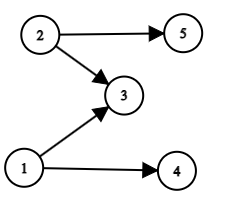
\includegraphics{img/graph.png}
        \caption{Unbinarizable graph}
        \label{fig04:3}
    \end{figure}
\end{example}

\begin{thm}\label{thm04:7}
    Theorem~\ref{thm04:5} transforms \emph{a planning problem} $\mathcal{P}$ with all \emph{methods} having \emph{linear ordering-constraints} into \emph{a planning problem} in $\text{NF}_{\geq 2}$ with all \emph{methods} having \emph{linear ordering-constraints}.
\end{thm}
\begin{proof}
    Theorem~\ref{thm04:5} includes two main parts: removing all \emph{empty methods} and \emph{unit-methods}. The elimination of \emph{unit-methods} does not have any effect on ordering because we need at least two tasks for \emph{an ordering-constraint}. We create new \emph{methods} without \emph{nullable} tasks which also deletes constraints containing these tasks. But because the ordering is linear even after the deletion of some elements (transitive closure from the definition) we do not create \emph{methods} with non-\emph{linear ordering-constraints}.
\end{proof}

\medskip\noindent
Before we start with the transformation of \emph{totally-ordered planning problems} we need to tidy up \emph{state-constraints}. So far, \emph{state-constraints} are defined on sets of subtasks, i.e., $before(p, U)$, $after(U, p)$, $between(U, p, V)$ with $U, V$ denoting subsets of subtasks, and $p$ denotes \emph{a propositional symbol}. \emph{TO planning problems} allow us to remove unnecessary tasks from sets $U, V$ leaving us with only one subtask. Hence, we abuse the notation to let $before(p, T)$ denote $before(p, \{ T \})$ with $T$ being \emph{a method's} subtask. Similarly, we will use this notation for $after$ and $between$ constraints. 

\begin{thm}\label{thm04:8}
    For each \emph{TO planning problem} there is \emph{an equivalent planning problem} with all \emph{state-constraints} having only one subtask.
\end{thm}
\begin{proof}
    Let us have \emph{a method} $T \rightarrow T_1, \dots, T_k \; [C], k \geq 1$, and a $before(p, U) \in C$. This constraint can be transformed to $before(p, T)$ such that $T \in U$ and $(\forall F \in (U - \{ T \})): T \prec F$. This can be done analogously for each $after(U, p)$ and $between(U, p, V)$ constraint. If the result $between(U, p, V)$ constraint is of a form $between(T, p, F)$ and $F \prec T$ holds then this whole constraint can be removed from the set of constraints as there are never states to test this constraint. 
\end{proof}

\medskip\noindent
Now, all \emph{TO} domains will implicitly have only \emph{state-constraints} described in Theorem~\ref{thm04:8}.

\medskip\noindent
In the following parts, we will try to convert general \emph{TO planning problems} into ones of a \emph{HTN-CNF}. Initially, we will compile away $between$ constraints because this type of \emph{state-constraint} spans throughout states which is undesirable. This behavior complicates the conversion because the \emph{HTN-CNF} has at most two tasks as subtasks. In this case, the $between(T_1, p, T_2)$ constraint is saying that the check is made before the application of the first \emph{action} to which $T_2$ decomposes, after the last \emph{action} to which $T_1$ decomposes, and also all states in between are checked. This means that the test is made in a single state after the last \emph{action} of $T_1$. This can be easily transformed to a single \emph{before-, after-constraint}. Complications with \emph{between-constraints} begin if we have at least three \emph{TO} subtasks $T_1 \prec T_2 \prec T_3$ and a $between(T_1, p, T_3)$ constraint. Having this, the check has to be made in (potentially) multiple states depending on a decomposition tree of \emph{a compound task} $T_2$. Transformation of this feature becomes difficult if we do not want to lose any information about \emph{a planning domain}.

\medskip\noindent
In~\cite{ondrckova2024empty} it is described how to get rid of $between$ constraints from \emph{TO planning problems} by adding a series of $before$ constraints. This conversion is false as it does not concern all states between subtasks but only states before the first \emph{action} to which potential \emph{compound tasks} decompose. Compiling away $between$ constraints is more complicated but not impossible. The Algorithm~\ref{alg04:1} below shows how to do it properly.

\medskip\noindent
In the following Algorithm~\ref{alg04:1}, we will create new \emph{compound tasks} that are derived from the existing ones. Let us have \emph{a compound task} $T$. A new \emph{compound task} $T_{\{p, q\}}$ (same name but with a suffix) denotes that in every possible decomposition tree starting from $T_{\{p, q\}}$ all \emph{methods} do not contain any $between$ constraints, and every \emph{primitive task network} derived from the $T_{\{p, q\}}$ holds \emph{propositional symbols} $\{p, q\}$ in every state. These new \emph{compound task} will be replaced in \emph{methods} containing $between$ constraints, and as a result, it will allow us to remove these constraints. Also, we will use the notation $before(Q, T)$ with $T$ being a task and $Q \subseteq P$ being a subset of \emph{propositional symbols}. $before(Q, T)$ is just an abbreviation for a $before(q_1, T), before(q_2, T), \dots$ where $q_i \in Q$.

\begin{algorithm}
    \caption{TO into TO without between-constraints}\label{alg04:1}
    \begin{algorithmic}[1]
        \Procedure {Main}{\emph{TO planning problem}: $\mathcal{P} = (s_0,\omega,\mathcal{D})$}
            \State $NewCT \gets \{\}$ \Comment{New \emph{Compound Tasks}}
            \While {$\mathcal{D}$ contains \emph{a method} $m$ with \emph{a between-constraint}}            
                \For {each \emph{compound task} $T$ in $subtasks(m)$ that is part of $\geq 1$ \emph{between-constraints}}
                    \State $PropSymbols \gets \{p: between(T, p, F) \; and \; T \prec t \prec F \}$
                    \If {$T_{PropSymbols}$ not in $NewCT$}
                        \State find \emph{methods} $m$ with $T = compound(m)$ and create new $m'=(T_{PropSymbols}, subtasks(m), constraints(m))$
                    \EndIf
                    \State swap all occurrences of $T$ with $T_{PropSymbols}$ in \emph{a method} $m$
                \EndFor

                \For {each task $t$ in $subtasks(m)$}
                    \State $PropSymbols \gets \{p: between(T, p, F) \; and \; T \prec t \prec F \}$
                    \State \Comment{if $PropSymbols = \emptyset$ then constraints are always satisfied}
                    \State add $before(PropSymbols, t)$, $after(t, PropSymbols)$ to $m$
                \EndFor
                
                \State remove all \emph{between-constraints} from $constraints(m)$

                \For {each $T_{symbols}$ in $subtasks(m)$ ($T_{symbols}$ not in $NewCT$)}
                    \State $NewCT \gets NewCT \cup T_{symbols}$
                    \State SearchCompoundTask($T_{symbols}$)
                \EndFor
            \EndWhile
        \EndProcedure
        \Procedure {SearchCompoundTask}{\emph{Compound task}: $T_{InputSymbols}$}
            \For {each \emph{method} $m$ with $T_{InputSymbols} = compound(m)$}
                \For {each task $t$ in $subtasks(m)$}
                    \State $PropSymbols \gets \{p: between(T, p, F) \; and \; T \prec t \prec F \}$
                    \State add $before(PropSymbols \cup InputSymbols, t)$ to $m$
                    \State add $after(t, PropSymbols \cup InputSymbols)$ to $m$
                \EndFor

                \For {each \emph{compound task} $T$ in $subtasks(m)$}
                    \State $PropSymbols \gets \{p: between(T, p, F) \; and \; T \prec t \prec F \}$
                    \If {$T_{PropSymbols \cup InputSymbols}$ not in $NewCT$}
                        \State find \emph{methods} $m$ with $T = compound(m)$ and create new $m'=(T_{PropSymbols \cup InputSymbols}, subtasks(m), constraints(m))$
                    \EndIf
                    \State swap all occurrences of $T$ with $T_{PropSymbols \cup InputSymbols}$ in $m$
                \EndFor

                \State remove all \emph{between-constraints} from $constraints(m)$

                \For {each $T_{symbols}$ in $subtasks(m)$ ($T_{symbols}$ not in $NewCT$)}
                    \State $NewCT \gets NewCT \cup T_{symbols}$
                    \State SearchCompoundTask($T_{symbols}$)
                \EndFor
            \EndFor
        \EndProcedure
    \end{algorithmic}
\end{algorithm}

\begin{thm}\label{thm04:9}
    For each \emph{TO planning problem} there is \emph{an equivalent planning problem} without any \emph{between-constraint}.
\end{thm}
\begin{proof}
    First of all, we will compile away \emph{between-constraints} of the neighboring tasks, i.e., tasks $T_1 \prec T_2$ such that no task $T_i$ exist with $T_1 \prec T_i$ and $T_i \prec T_2$. As was said before, these constraints can be interchanged to a single \emph{before-constraint}. \emph{Between-constraints} of a form $between(T_i, p, T_i)$ or $between(T_j, p, T_i)$ with $T_i \prec T_j$ are pointless and can be removed without any loss of information.
    
    The idea of the Algorithm~\ref{alg04:1} is to remove \emph{between-constraints} \emph{method} by \emph{method} with a procedure that might remind us of Depth-first search (DFS). Suppose a method \( M \) includes at least one \emph{between-constraint}. In every valid \emph{solution} of the \emph{planning problem} \(\mathcal{P}\) that employs \( M \) during the planning phase, there must exist a consecutive \emph{sub-plan} that is decomposed from the \( \text{compound}(M) \) and contains the \emph{propositional symbol} specified in the constraint.

    If we want to remove $between(T, p, F)$ constraint then we must ensure that all decompositions (even those with cycles) of all \emph{compound tasks} between $T$ and $F$ (with respect to \emph{TO}) hold \emph{propositional symbol} $p$.
    
    An algorithm is split into two distinct parts: the while-loop (3) in the \texttt{Main} function and a recursive function \texttt{SearchCompoundTask} (23). The main cycle removes all \emph{between-constraints} from a single \emph{method} per iteration meanwhile not creating any new \emph{between-constraints}. All \emph{compound tasks} that are mentioned in \emph{between-constraints} are substituted with new \emph{compound tasks} that are stored in an auxiliary set \texttt{NewCT} (2). If a substituted \emph{compound task} is already stored in \texttt{NewCT} then we do not have to recursively search this task with \texttt{SearchCompoundTask} function (17, 38). On the contrary, if the task is not searched then we need to create new \emph{methods} so that tasks from other \emph{methods} cannot be decomposed via \emph{methods} designed for the substituted tasks (7, 33).

    The recursive procedure \texttt{SearchCompoundTask} looks for all \emph{methods} that decompose the input \emph{compound tasks} and append constraints so that the \emph{propositional symbols} are checked in all states concerning the subtasks (27, 28). Also, the recursive procedure removes all \emph{between-constraints} during the search (35), so they are not found in the main while-loop.


    There is a finite number of \emph{propositional symbols}, \emph{methods}, \emph{compound tasks}, and new \emph{compound tasks} in \texttt{NewCT}. Therefore, the algorithm will not fall into an infinite cycle, and gradually all \emph{between-constraints} will be removed.
\end{proof}

\begin{thm}\label{thm04:10}
    For each \emph{TO planning problem} that does not generate empty \emph{plan} as a \emph{solution}, there is \emph{an equivalent planning problem} without \emph{empty methods}.
\end{thm}
\begin{proof}
    First, we will remove all \emph{between-constraints} with the Theorem~\ref{thm04:9}.

    Similarly to Theorem~\ref{thm04:5}, we will need to find all \emph{nullable tasks} in \emph{a planning problem} and create new \emph{methods} without these tasks. The difficult part is handling the \emph{before-, after-constraints} which need to be checked eventually. \emph{A nullable task} may have many different series of decompositions that lead to an empty set of tasks. Each of these decompositions may have different constraints that need to be checked. For this purpose, we will use a function $Nullifies(T)$ that accepts a \emph{nullable compound task} and returns a set of sets of \emph{propositional symbols}. Each element of the function's output represents one possible way of how we can decompose this \emph{compound task} and which \emph{propositional symbols} need to be checked.

    We will find all values of the function $Nullifies$ in the following inductive manner. \textbf{Base:} for each $T \rightarrow \varepsilon \; [\{\}]: Nullifies(T) = \{\{\}\}$. \textbf{Induction:} having $T \rightarrow T_1, \dots, T_k \; [C], \; k \geq 1$ with subtasks containing only \emph{nullable compound tasks} we extend $Nullifies(T) = Nullifies(T) \; \cup \; \{\{\text{propositional symbols mentioned in} \; C\} \\ \cup propSym_1 \cup \dots \cup propSym_k\}$ where $propSym_i \in Nullifies(T_i)$. The induction part is repeated until there is a new unique combination of \emph{propositional symbols} that is not mentioned in $Nullifies(T)$ with some \emph{nullable compound task} $T$ and some \emph{method} $T \rightarrow T_1, \dots, T_k \; [C], \; i \geq 1$.

    It can be easily seen that $T$ is \emph{nullable} if and only if $Nullifies(T) \neq \emptyset$ (after we have found all values). \emph{The compound task} in \emph{the initial task network} is never \emph{nullable} as stated in the theorem. This feature will be used in the second part of the \emph{empty method} elimination.

    At this point, all \emph{empty methods} can be removed from the \emph{planning domain}.

    Now, for the final part, we will append new \emph{methods} with/without \emph{nullable tasks} to the \emph{planning problem}, similarly to Theorem~\ref{thm04:5}. Suppose \emph{a method} contains $i$ \emph{nullable tasks} in $subtasks$. Without loss of generality, \emph{nullable tasks} will be $T_1, \dots, T_i$. There will be $(|Nullifies(T_1)| + 1) \times \dots \times (|Nullifies(T_i)| + 1)$ new \emph{methods}, some of them might be identical. For each such combination, we will create a new \emph{method} without (some) \emph{nullable tasks}. Constraints mentioning deleted tasks are removed from the set of constraints. If we want to remove \emph{a nullable task} $T_j$ then we need to find the closest task that is not removed from the \emph{method} and append new \emph{state-constraints} to \emph{the method}. If the non-removed task $T_k$ holds $k < j$ then we create new constraints: $after(T_k, p_1), after(T_k, p_2), \dots$, where $p_i \in PropSymbols \in Nullifies(T_j)$. On the other hand, if $k > j$ then we append $before(T_k, p_1), before(T_k, p_2), \dots$ to the set of \emph{method's} constraints. It might happen that all $subtasks(M)$ of \emph{a method} $M$ are \emph{nullable}, in this case, we do not create new \emph{empty method} because $compound(M)$ will be removed from \emph{methods} that contain $compound(M)$ as a subtask. As was stated before, \emph{initial task network} is never \emph{nullable}, thus we do not need to handle this awkward situation.
\end{proof}

\begin{thm}\label{thm04:11}
    For each \emph{TO planning problem} there is \emph{an equivalent planning problem} without any \emph{after-constraints}.
\end{thm}
\begin{proof}
    \emph{TO planning problems} allow us to shift any \emph{after-constraint} to the succeeding task. So, \emph{an after-constraint} is changed to \emph{before-constraint}. This transformation is valid with only one exception. If \emph{the after-constraint} targets the last task with respect to \emph{TO} then \emph{an after-constraint} cannot be shifted to the following task because such task does not exist in a set of \emph{method's} $subtasks$. One might think that we can compile this feature away using the cooperation with other \emph{methods}. Still, it can happen that the targeted task will be the last \emph{action} in \emph{the solution} which means that the check will be evaluated in a state after the execution of all \emph{actions} in \emph{the plan}. Therefore, in this case, we cannot shift \emph{an after-constraint} so easily. What we can do is to create a new \emph{compound task} $T_{empty}$ with one \emph{empty method}. Then, this task can be inserted at the end of \emph{a method} and problematic \emph{after-constraints} can be shifted to the $T_{empty}$.

    Symmetrically, we can transform all \emph{before-constraints} to the equivalent \emph{after-constraints}.
\end{proof}

\begin{thm}\label{thm04:12}
    For each \emph{TO planning problem} that does not generate empty \emph{plan} as a \emph{solution}, there is \emph{an equivalent planning problem} in \emph{HTN-CNF}.
\end{thm}
\begin{proof}
    The proof is akin to proofs of Theorems~\ref{thm04:5}~\ref{thm04:6} with some extra steps to handle \emph{state-constraints}. At the beginning, we will use Theorem~\ref{thm04:9} to remove all \emph{between-constraints}. Afterwards, we will use Theorem~\ref{thm04:10} to remove all \emph{empty methods} which does not create any new \emph{between-constraints}. Now we need to handle \emph{unit methods}. We will find all \emph{unit pairs} which is identical to the proof to the Theorem~\ref{thm04:5}. Analogous to the process of discarding \emph{empty methods} \emph{unit pairs} might have different decompositions which lead to different sets of constraints. As for \emph{empty methods}, we will find all such combinations of \emph{unit pairs} with sets of constraints with the help of an auxiliary function $Nulifies(T, F)$ with $(T, F)$ being an \emph{unit pair}. \textbf{Base:} for each \emph{unit method} $T \rightarrow F \; [C]$: $Nullifies(T, F) = \{C\}$ (if there are multiple \emph{unit methods} with identical \emph{compound tasks} but with different constraints then each set of constraints is added separately). \textbf{Induction:} having \emph{a unit pair} $(T, F)$ and \emph{a unit method} $F \rightarrow H \; [C]$: $Nullifies(T, H) = Nullifies(T, H) \; \cup \; \{constr_t \cup constr_h \; | \; (\forall constr_t \in Nullifies(T, F)) \; and \; (\forall constr_h \in Nullifies(F, H))\}$. Hence, for each \emph{unit pair} $(T, F)$ and for each \emph{non-unit method} $F \rightarrow F_1, \dots, F_k \; [C]$ we create new \emph{methods} for each set of constraints in $Nullifies(T, F)$. New \emph{method} is of a form $T \rightarrow F_1, \dots, F_k \; [C \cup newC]$ where $newC$ are newly produced constraints from $newConstr \in Nullifies(T, F)$. $newC = \{before(p, F_1) \; | \; before(p, X) \in newConstr\} \cup \{after(F_k, p) \; | \; after(X, p) \in newConstr\}$. After that, we can remove all \emph{unit methods}.

    For each \emph{method} with multiple subtasks with at least one \emph{primitive task} as a subtask, we substitute \emph{a primitive task} $a$ with \emph{a compound task} $T_a$. All constraints targeting $a$ are interchanged with constraints targeting $T_a$. We also create a new \emph{method} $T_a \rightarrow a \; [\{\}]$. Now, our \emph{planning problem} is in $\text{NF}_{\geq 2}$. To finish the proof we need to divide long \emph{methods}.

    For each \emph{method} $T \rightarrow T_1, \dots, T_k \; [C], \; k \geq 3$ we produce $k - 2$ $C_i$ \emph{compound tasks}, and construct new \emph{methods} $T \rightarrow T_1, C_1 \; [\{T_1 \prec C_1\} \; \cup \; \{\text{all \emph{state-constraints}} \\ \text{targeting} \; T_1\}]$, $C_1 \rightarrow T_2, C_2 \; [\{T_2 \prec C_2\} \; \cup \; \{\text{all \emph{state-constraints} targeting $T_2$}\}]$, $\dots$, $C_{k-2} \rightarrow T_{k-1}, T_k \; [\{T_{k-1} \prec T_k\} \; \cup \; \{\text{all \emph{state-constraints} targeting $T_{k-1}, T_k$}\}]$.
\end{proof}

\begin{defn}\label{def04:18}
    A \emph{hierarchical planning problem} $\mathcal{P} = (s_0,\omega,\mathcal{D})$ is said to be in \emph{HTN-GNF~\cite{gnf}} if all of its methods are of the form: $T \rightarrow a, T_1, T_2, \dots, T_i \; [C], \; i \geq 0$; where $T, T_i$ are \emph{compound tasks}, and $a$ is a \emph{primitive task}. 
\end{defn}

\begin{thm}\label{thm04:13}
    For each \emph{TO planning problem} in \emph{HTN-CNF} there is \emph{an equivalent planning problem} in \emph{HTN-GNF}.
\end{thm}
\begin{proof}
    We assume that \emph{the planning problem} does not contain any \emph{between-constraints} as they can be easily eliminated in \emph{HTN-CNF}. The practice is to be found above.

    The proof follows the~\cite{gnf} (Chapter 7.1) with the addition of HTN specifics. Initially, we rename \emph{compound tasks} to $A_1, A_2, \dots, A_n$ in some ascending order (and substitute these new tasks in constraints). \emph{The compound task} in \emph{the initial task network} is renamed to $A_1$. Our next goal is to modify \emph{methods} such that $A_i \rightarrow A_j, \alpha \; [C] \implies i > j$ where $T_j$ is the first \emph{compound task} with respect to ordering, and $\alpha$ is a set of both \emph{primitive and compound tasks}.

    Starting from the $A_1$ and proceeding to \emph{the compound task} with the highest index, we find all \emph{methods} of a form:  $A_i \rightarrow A_j, \alpha \; [C], \; i > j$. For each such \emph{method} we construct new \emph{methods} replacing $A_j$ with the $subtasks(M)$ such that $compound(M) = A_j$ for \emph{methods} $M$. Constraints $C$ are unioned with the $constraints(M)$, transitive closure of \emph{ordering-constraints} between $subtasks(M)$ and $\alpha$ is made, and all \emph{state-constraints} targeting $A_j$ are substituted as follows: each $before(p, A_j)$ is substituted with $before(p, A_x)$ such that $A_x$ is the first task in $subtasks(M)$, and each $after(A_x, p)$ is substituted with $after(A_x, p)$ such that $A_x$ is the last task in $subtasks(M)$. By repeatedly using this technique we obtain \emph{methods} $A_i \rightarrow A_j, \alpha \; [C], \; i \leq j$, ones starting with \emph{an action}, or ones starting with a new \emph{compound symbol} $Z$. After that, we need to remove left recursion from our new \emph{methods} for $A_i$, that is $A_i \rightarrow A_i, \alpha \; [C]$. Doing so is more difficult than in \emph{CFG} because we need to handle \emph{state-constraints} properly. First, we need to slightly modify \emph{methods' constraints} containing left recursion. For each \emph{method} $A_i \rightarrow A_i, \alpha \; [C]$ ($\alpha$ is always nonempty) we find all \emph{after-constraints} targeting $A_i$ and shift them to the succeeding task resulting in \emph{before-constraint} on the first task in $\alpha$ (with respect to ordering). We can do this because our domain is \emph{TO} and the check will be made in the same state. Afterward, we will construct a $\Omega$ – set of sets with \emph{propositional symbols} where each element is a union of \emph{propositional symbols} found in \emph{a before-constraints} targeting the first task in \emph{a method} with left recursion of $A_i$. Now we need to find all \emph{methods} with $compound(M) = A_i$ and separate them into two groups (with/without left recursion):

    \[
        A_i \rightarrow A_i, \alpha_1 \; [C_1] \; | \; \dots \; | \; A_i, \alpha_m \; [C_m],
    \]

    \[
        A_i \rightarrow \beta_1 \; [C_1] \; | \; \dots \; | \; \beta_p \; [C_p].
    \].

    With these two groups, we eliminate left recursion by introducing new \emph{compound task} $Z$, and substituting these \emph{methods} with:

    \begin{gather*}
        A_i \rightarrow \beta_i \; [C_i \cup \{before(Q, \beta_i) \; | \; Q \; \text{is a union of some elements from} \;\Omega\}] \; | \; \beta_i, Z \\ [C_i \cup \{before(Q, \beta_i) \; | \; Q \; \text{is a union of some elements from} \;\Omega \} \cup \{\beta_i \prec Z\}], \\ 1 \leq i \leq  p, \\ \\
        Z \rightarrow \alpha_i \; [C_i] \; | \; \alpha_i, Z \; [C_i \cup \{\alpha_i \prec Z\}], 1 \leq i \leq m.
    \end{gather*}

    In the new \emph{methods} the former set of constraints $C_i$ is restricted to relevant tasks. Doing so, we can move on to the next task $A_{i + 1}$ and repeat the process.

    At this point, $A_i \rightarrow A_j, \alpha \; [C] \implies i > j$ holds. For the last part, we will modify $A_i \rightarrow A_j, \alpha \; [C]$ for $i = n - 1, n - 2, \dots, 1$ so the \emph{methods} start with \emph{an action}, and at the same time we modify new $Z$ \emph{methods}. The final modification is analogous to the one in the third paragraph.
\end{proof}




% \section{many different formalisms and languages}
% look for features that can be transformed or deleted \\
% \cite{hddl}=list of formalisms with publication


\chapter*{Conclusion}

\noindent
To sum up, the main purpose of this thesis was to make a brief introduction to the field of planning and to explore some aspects that can be later employed in other types of related work. Starting from classical planning which can be expressed in different ways and lasting with hierarchical planning, HTN to be precise. The theory of HTN is not yet unified, therefore we can find different definitions and understandings about this topic in various publications. 

\medskip\noindent
One of the goals was to set proper boundaries via combinations of definitions from varying sources. By doing so, we could describe, compare, and analyze HTN semantics with the subtle goal of handling empty methods that are not handled accurately in plenty of similar papers. Difficulties start to appear if we want to use constraints that are bound to states. Also, new types of HTN semantics were introduced.

\medskip\noindent
In the last chapter of the thesis, we tried to find transformations of HTN models that might be suitable within some context. Most transformations were inspired by the theory of Automata and Grammars, yet they need a significant amount of extension as HTN models allow partially-ordered domains and state-constraints.    

\addcontentsline{toc}{chapter}{Conclusion}


%%% Bibliography
%%% Bibliography (literature used as a source)
%%%
%%% We employ bibTeX to construct the bibliography. It processes
%%% citations in the text (e.g., the \cite{...} macro) and looks up
%%% relevant entries in the bibliography.bib file.
%%%
%%% The \bibliographystyle command selects, which style will be used
%%% for references from the text. The argument in curly brackets is
%%% the name of the corresponding style file (*.bst). Both styles
%%% mentioned in this template are included in LaTeX distributions.

\bibliographystyle{plainnat}    %% Author (year)
% \bibliographystyle{unsrt}     %% [number]

\renewcommand{\bibname}{Bibliography}

%%% Generate the bibliography. Beware that if you cited no works,
%%% the empty list will be omitted completely.

\bibliography{bibliography}

%%% If case you prefer to write the bibliography manually (without bibTeX),
%%% you can use the following. Please follow the ISO 690 standard and
%%% citation conventions of your field of research.

% \begin{thebibliography}{99}
%
% \bibitem{lamport94}
%   {\sc Lamport,} Leslie.
%   \emph{\LaTeX: A Document Preparation System}.
%   2nd edition.
%   Massachusetts: Addison Wesley, 1994.
%   ISBN 0-201-52983-1.
%
% \end{thebibliography}


%%% Figures used in the thesis (consider if this is needed)
\listoffigures

%%% Tables used in the thesis (consider if this is needed)
%%% In mathematical theses, it could be better to move the list of tables to the beginning of the thesis.
%\listoftables

%%% Abbreviations used in the thesis, if any, including their explanation
%%% In mathematical theses, it could be better to move the list of abbreviations to the beginning of the thesis.
\chapwithtoc{List of Abbreviations}
\noindent
AI – Artificial Intelligence \\
BFS – Breadth-First Search \\
CFG – Context-free Grammar \\
ChNF – Chomsky Normal Form \\
DAG – Directed Acyclic Graph \\
DFA – Deterministic Finite Automaton \\
DFS – Depth-First Search \\
GNF – Greibach Normal Form \\
HDDL – An Extension to PDDL for Expressing Hierarchical Planning Problems \\
HTN – Hierarchical Task Network \\
LLM – Large Language Models \\
PO – Partially-ordered \\
TO – Totally-ordered

%%% Doctoral theses must contain a list of author's publications
\ifx\ThesisType\TypePhD
\chapwithtoc{List of Publications}
\fi

%%% Attachments to the thesis, if any. Each attachment must be referred to
%%% at least once from the text of the thesis. Attachments are numbered.
%%%
%%% The printed version should preferably contain attachments, which can be
%%% read (additional tables and charts, supplementary text, examples of
%%% program output, etc.). The electronic version is more suited for attachments
%%% which will likely be used in an electronic form rather than read (program
%%% source code, data files, interactive charts, etc.). Electronic attachments
%%% should be uploaded to SIS. Allowed file formats are specified in provision
%%% of the rector no. 72/2017. Exceptions can be approved by faculty's coordinator.
\appendix
\chapter{Attachments}

\section{First Attachment}

\subsection*{NAME}
\textbf{htn-transformator} - a command-line program that demonstrates some of the transformations mentioned in this text.

\subsection*{SYNOPSIS}
\texttt{htn-transformator -i INPUTFILE [--between|--empty|--tocnf]} \\
\texttt{[-o OUTPUTFILE]}

\subsection*{DESCRIPTION}
\texttt{htn-transformator} is a utility designed to apply specific transformations to HTN planning domains.

\subsection*{OPTIONS}
\begin{description}
\item[-i INPUTFILE]
Specifies the input file containing the HTN data. This option is mandatory.

\item[--between]
Removes all between constraints from the input planning domain.

\item[--empty]
Removes all between constraints and empty methods from the input planning domain.

\item[--tocnf]
Transforms the input planning domain into the HTN-ChNF.

\item[-o OUTPUTFILE]
Specifies an optional output file to save the result. If this option is omitted, the output is displayed to stdout.
\end{description}

\end{document}
